\documentclass[11pt]{article}

% ------------------------------------------------------------------
% Packages
% ------------------------------------------------------------------
\usepackage[utf8]{inputenc}
\usepackage[T1]{fontenc}
\usepackage[margin=1in]{geometry}
\usepackage{amsmath}
\usepackage{amssymb}
\usepackage{booktabs}
\usepackage{array}
\usepackage{graphicx}
\usepackage{caption}
\usepackage{enumitem}
\usepackage{hyperref}
\usepackage{textcomp}
\usepackage{soul}

\hypersetup{
    colorlinks=true,
    linkcolor=black,
    citecolor=black,
    urlcolor=blue,
    pdftitle={Time Series Analysis of U.S. Daily Wheat, Corn, and Soybeans Futures Prices},
    pdfauthor={Anthony Le}
}

% Hanging-indent style for the reference list
\newenvironment{references}
  {\begin{list}{}{%
      \setlength{\leftmargin}{0.4in}%
      \setlength{\itemindent}{-0.4in}%
      \setlength{\itemsep}{0.6\baselineskip}%
      \setlength{\parsep}{0pt}%
  }}
  {\end{list}}

\setlength{\parindent}{0pt}
\setlength{\parskip}{0.6\baselineskip}

% ------------------------------------------------------------------
% Title
% ------------------------------------------------------------------
\title{\textbf{Time Series Analysis of U.S. Daily \\ Wheat, Corn, and Soybeans Futures Prices}}
\author{\textbf{Anthony Le} \\[0.3em] \normalsize Department of Mathematics, Denison University}
\date{December 17, 2024}

\begin{document}

\maketitle

\begin{abstract}
\noindent This paper analyzes daily futures prices for wheat, corn, and soybeans traded on the Chicago Board of Trade from January 2000 to December 2024, using ARIMA, GARCH, multivariate GARCH, and ARIMAX models to characterize trends, volatility, and interdependence across the three markets. Spectral analysis reveals no significant seasonality in prices or trading volumes, consistent with these derivatives reflecting evolving market expectations rather than fixed calendar effects. The best-fitting ARIMA models leave residuals that are stationary but not independent or normal, limiting their forecasting reliability; univariate GARCH models fit to returns fare better on residual diagnostics but still yield poor out-of-sample cross-validation performance (negative R-squared values). Multivariate GARCH estimates reveal strong, persistent correlations across all three commodities, particularly between wheat and corn, motivating ARIMAX specifications that incorporate a correlated commodity's price as an exogenous regressor. While these results do not yield production-ready forecasting models, they clarify the volatility dynamics and cross-commodity linkages relevant to portfolio construction and risk management in agricultural derivatives markets.
\end{abstract}

% ==================================================================
\section{Introduction}
% ==================================================================

In the modern economy, the agricultural commodities market is integral to global trade and economic stability, providing food, feed, and raw materials for a diverse range of industries. However, prices in this sector are highly volatile due to weather-dependent production, geopolitical events, and macroeconomic fluctuations. Futures markets for commodities like wheat, corn, and soybeans provide a vital platform for buyers and sellers to trade standardized contracts for future delivery. These markets primarily facilitate investment opportunities for speculators and hedgers against price volatility, especially during times of uncertainty (Pawlowski, Rechtsteiner, and Joscha Schabram, 2024).

As some of the most traded agricultural commodities, wheat, corn, and soybeans have their prices that depend highly on market supply and demand, weather events, and macroeconomic conditions. In fact, their futures prices are crucial indicators of market expectations and, thus, a valuable tool for risk management among stakeholders (M. Ates, Marsh, and Hubbs, 2024).

This paper focuses on the analysis of daily futures prices for wheat, corn, and soybeans from January 2000 to the end of December 2024. Using advanced time series methodologies, this writer hopes to identify potential key trends and volatility in these markets, explore the interdependence among futures prices of these commodities, and produce forecasts of future trading prices, especially for December 2024. In essence, this paper aspires to contribute meaningful insights into market dynamics and develop forecasting models that will be beneficial for professional applications in finance.

% ==================================================================
\section{Methods}
% ==================================================================

\subsection{Working Data}

\subsubsection{Data Acquisition \& Wrangling}

The data analyzed in this project consist of daily closing prices and trading volumes for wheat, corn, and soybean futures contracts traded on the Chicago Board of Trade (CBOT) between January 3, 2000, and December 5, 2024, retrieved in CSV format from Investing.com and Yahoo Finance.

The process of data wrangling takes place in both Excel and RStudio, after which 6,314 observations were retained in an xts object, representing data on closing prices and trading volumes for 6,314 trading days on which prices of all three commodities futures were available. With between 50 and 70 missing values on the trading volumes of each contracts randomly scattered throughout the timeframe, a process of data interpolation based on linear approximations was performed to handle missing data.

\subsubsection{Understanding Futures Contract}

In the financial market, a futures contract is a legally binding agreement to buy or sell a specific commodity, asset, or security at a predetermined price on a specified date or time in the future. Futures contracts are standardized for quality and quantity to facilitate trading on a futures exchange. Unlike the stock market, most futures markets are open nearly 24 hours a day, from Sunday evening to Friday afternoon, with only a few exceptions that have unique trading hours. More information about futures contracts can be found \href{https://www.investopedia.com/terms/f/futurescontract.asp}{here} or other online resources.

In this project, each commodity futures contract of interest represents 5,000 bushels ($\sim$136 metric tons) of the respective commodity, with prices quoted in U.S. cents per bushel. This granularity enables tracking of even minor price fluctuations, as the minimum price change is a quarter of one cent (\$0.0025) per bushel. For visualization and interpretation purposes, prices are shown in U.S. dollars in this project.

\subsubsection{Argument of Sample \& Potential Issues}

As the data is sourced from the Chicago Board of Trade (CBOT), representing a segment of the broader futures market with other significant exchanges, such as NYSE Euronext (Euronext), Kansas City Board of Trade (KCBT), or Minneapolis Grain Exchange (MGEX), it reflects only a portion of global trading activity. The dataset is, therefore, considered a sample of the larger population of futures contracts across different US exchanges and may even introduce sampling bias if market dynamics differ significantly across exchanges.

Moreover, this writer also acknowledges that trading volume data, although valuable, can be prone to reporting discrepancies or missing values, thereby complicating its use in analysis. Having these concerns in mind, this paper aims to apply robust preprocessing steps, cross-validation techniques, and interpretative care in the analysis to mitigate potential biases and limitations.

\subsection{Time Series Analysis}

\subsubsection{Assumption and Validation}

To conduct a rigorous statistical analysis of U.S. daily wheat, corn, and soybean prices, it is essential to assume that each account in the data is independent of the others. The following paragraphs outline the general approach to finding the best models for available data.

Before fitting any model, we will visualize the data with a time series plot and, if appropriate, compute the Autocorrelation Function (ACF) and Partial Autocorrelation Function (PACF) plots to understand the underlying patterns. We will then perform several stationarity tests, including the Augmented Dickey-Fuller (ADF), Phillips-Perron (PP), Kwiatkowski-Phillips-Schmidt-Shin (KPSS), and the Elliott-Rothenberg-Stock (ERS) tests. To identify potential significant frequency, spectral analysis with bootstrapping confidence intervals will also be performed before model fitting steps. More information on these tests and techniques will be available in the Appendix.

After fitting the models, we will validate their effectiveness by plotting the fitted values with the original data and then analyzing the residua through time series plots, density plots, as well as a series of other statistical tests. At this stage, we will check for randomness, stationarity, independence, normality, and linearity of the residuals as relevant. When comparing models, we will utilize the Akaike Information Criterion (AIC), Bayesian Information Criterion (BIC), and R-squared values (for linear models). While, in general, lower AIC and BIC values, along with a higher R-squared value, indicate a better-fitting model, we have to consider the following relationships:

\begin{itemize}
\item To trust R-Squared values, residuals should primarily be random, independent, and ideally stationary.
\item To trust AIC and BIC values, the residuals must be stationary and independent.
\item To trust p-values and confidence intervals, residuals should exhibit independence, linearity (in linear regression models), and normality (for large samples, normality can be relaxed due to the Central Limit Theorem, but in small samples, non-normal residuals can lead to inaccurate inferences).
\item To trust forecasts, residuals need to be stationary, random, and independent.
\end{itemize}

For validation, we will implement a cross-validation approach by excluding data from October 2024, training our models with the available data up to September 2024, and subsequently comparing the models' predictions against actual closing prices for the last three months of 2024. Finally, if the model satisfies ideal assumptions, we will forecast futures prices for one month into the future, i.e., December 2024.

\subsubsection{Seasonality Detection}

Leveraging techniques of Seasonal-Trend decomposition using LOESS (STL), non-parametric smoothing, and spectral analysis, we can identify potentially important frequencies that correspond to elements of seasonality in price fluctuations of our futures contracts. However, it is noteworthy that, unlike many economic or environmental time series that show predictable seasonal fluctuations (like retail sales or temperature), futures prices primarily reflect market expectations about future events, which can be highly dynamic and thus may not easily be categorized into regular seasonal patterns.

\subsubsection{ARIMA \& ARIMAX Models}

Autoregressive Integrated Moving Average (ARIMA) models and ARIMA with exogenous inputs (ARIMAX) models can help identify and leverage the interdependence of current and lagged observations, as well as their relationship with an external variable. Mathematically, an ARIMAX (p,d,q) model can be written as:

\begin{equation}
y_{t} = c + \beta x_{t} + \sum_{i=1}^{p}\phi_{i}\,y_{t-i} + \sum_{i=1}^{q}\theta_{i}\epsilon_{t-i} + \epsilon_{t},
\end{equation}

where $y_{t}$ is the dependent variable (if $d = 0$), or $y_{t} = \Delta z_{t}$ with $z_{t}$ being the dependent variable (if $d = 1$).

\subsubsection{GARCH Models}

Generalized AutoRegressive Conditional Heteroskedasticity (GARCH) models are commonly used to help predict the volatility of returns on financial assets. In this analysis, this statistical model helps analyze the returns on each of the three commodities' futures contracts over time. In general, a GARCH(p,q) model would refer to a time series whose values can be given by $r_{t} = \sigma_{t}\epsilon_{t}$ with $\epsilon_{t} \sim N(0,1)$ and whose variance can be given by

\begin{equation}
\sigma_{t}^{2} = \omega + \sum_{i=1}^{p}\alpha_{i}r_{t-1}^{2} + \sum_{i=1}^{q}\beta_{i}\sigma_{t-i}^{2}.
\end{equation}

By trying to fit the best GARCH models with appropriate residual distributions, we hope to produce trustworthy forecasts for future pricing of these derivatives (i.e. financial instruments whose value is derived from an underlying asset, such as stock, bond, interest rate, or, in this case, commodity).

\subsubsection{Multivariate GARCH Models}

According to Ghalanos (2022), the generalization of univariate GARCH models to the multivariate domain is conceptually simple. Consider the stochastic vector process, $x_{t}\ \{t = 1, 2, ...T\}$ of financial returns with dimension $N \times 1$ and mean vector $\mu_{t}$\footnote{The mean vector may for example be derived from a VAR model or may simply represent the unconditional means of the financial returns.}, given the information set $I_{t-1}$:

\begin{equation}
x_{t}|I_{t-1} = \mu_{t} + \epsilon_{t},
\end{equation}

where the residuals of the process are modelled as:

\begin{equation}
\epsilon_{t} = H_{t}^{1/2}z_{t},
\end{equation}

and $H_{t}^{1/2}$ is a $N \times N$ positive definite matrix such that $H_{t}$ is the conditional covariance matrix of $x_{t}$\footnote{One way to obtain the square root matrix is through the singular value decomposition of $H_t$.}, and $z_{t}$ is an $N \times 1$ i.i.d. random vector, with centered and scaled first two moments:

\begin{equation}
E[z_{t}] = 0 \quad \text{and} \quad Var[z_{t}] = I_{N},
\end{equation}

with $I_{N}$ denoting the identity matrix of order N. The conditional covariance matrix $H_{t}$ of $x_{t}$ may be defined as:

\begin{equation}
Var[x_{t}|I_{t-1}] = Var_{t-1}[x_{t}] = Var_{t-1}[\epsilon_{t}] = H_{t}^{1/2}Var_{t-1}[z_{t}](H_{t}^{1/2})' = H_{t}.
\end{equation}

The usual trade-off of model parametrization and dimensionality clearly applies here, with the fully parameterized models offering the richest dynamics at the cost of increasing parameter size, making it unfeasible for modelling anything beyond a couple of assets. However, for this analysis, this model is sufficient for estimating and forecasting the correlation between each pair of futures contracts. This information is crucial to constructing portfolios that minimize correlated risks and maximize risk-adjusted returns.

\subsubsection{Cross Validation \& Forecasting}

To validate the effectiveness of the models we fit, for each series of data, the best fitting model will be cross-validated with the actual data from October 1 to December 5, 2024 (47 observations). We will compute the R-Squared values of the forecast and actual data. If the results are significant, we will continue to train the data on all available data (up to December 5, 2024) and try to predict the prices of futures contracts for the rest of the year.

\subsubsection{Special Functions}

To facilitate various analyses and avoid repetition in the codes, self-defined functions are introduced in R to streamline various processes, and they include:

\begin{itemize}
\item \texttt{check\_stationarity()}: This function performs stationarity tests (ADF, PP, KPSS, ERS) and summarizes the results in a user-friendly table.
\item \texttt{diff\_plots()}: This function plots the time series and generates both ACF and PACF plots of the data, helping assess autocorrelation visually.
\item \texttt{model\_summary\_table()}: These functions summarize the key metrics of fitted models, including R2, AIC and BIC values, to facilitate comparison.
\item \texttt{check\_normality\_residuals()}: This function evaluates the residuals from fitted models through a series of different tests to ensure they conform to normality assumptions.
\item \texttt{ts\_summary\_table()}: This function summarizes key characteristics of time series data.
\item \texttt{calculate\_r2()}: This function computes the R-Squared for model predictions against actual data.
\end{itemize}

% ==================================================================
\section{Results and Conclusions}
% ==================================================================

\subsection{Descriptive Analysis}

While wheat, corn, and soybeans production may experience seasonal variations in production, demand, and prices, their futures contracts come in as stabilizers, helping both the producers and consumers secure a purchase price months into the future. Hence, the prices of such derivatives tend to move along the larger macroeconomic movements in the financial markets, rather than due to fixed seasonal fluctuations. Figure 1 illustrates the prices and volumes of wheat, corn, and soybeans futures since January 2000.

From the figure, it is apparent that there is no clear yearly, quarterly, or monthly seasonality in both prices and volumes of these derivatives. Historically, while soybean futures have been consistently traded at higher prices than the other two assets, corn futures are most commonly traded with the highest volumes. All of them, regardless, experience relatively similar shocks over the last two decades, with the price hikes during the Great Recession and the COVID-19 pandemic being most significant.

\subsection{Seasonality \& Spectral Analysis}

Due to the non-seasonality of the data, functions such as ``decompose()'' or ``stl()'' could not be run, but they printed ``time series has no or fewer than 2 periods.'' This aligns with our observations from above and the economic intuition associated with derivatives markets. Moreover, with the spectrums of both differenced and returns data not showing any significant frequencies (Figure 2), we are now positive that there is no clear seasonality in the data. However, using ``ksmooth()'', we were able to expose some longer-term trends in these markets (Figure 3). From the visualization, it appears sensible to believe that even with these longer-term trends, there does not seem to be any function of time that can capture the fluctuations in the prices of these derivatives well.

\subsection{ARIMA Models}

\textbf{\emph{Wheat Futures}}

In terms of ARIMA models, the best model we can get for wheat futures prices is an ARIMA(1,1,3) with the following mathematical expression:

\begin{equation}
\Delta y_{t} = 0.4723\,\Delta y_{t-1} - 0.4298\,\epsilon_{t-1} - 0.0275\,\epsilon_{t-2} - 0.0485\,\epsilon_{t-3} + \epsilon_{t}
\end{equation}

This equation implies that the price difference in wheat futures today depends on the price difference of the day before, as well as the variability in contract prices of the previous three days and of today. The residuals of this model seem stationary, but are not independent nor normal, making it untrustworthy to be used for forecasting. Refer to Figure 4.

\textbf{\emph{Corn Futures}}

Meanwhile, the best ARIMA model we can get for corn futures prices is an ARIMA(0,1,3) with the following mathematical expression:

\begin{equation}
\Delta y_{t} = 0.0224\,\epsilon_{t-1} - 0.0336\,\epsilon_{t-2} + 0.0306\,\epsilon_{t-3} + \epsilon_{t}
\end{equation}

This equation implies that the price difference in corn futures today depends purely on the variability in contract prices of the previous three days and of today. The residuals of this model seem stationary, but are not independent nor normal, making it untrustworthy to be used for forecasting. Refer to Figure 5.

\textbf{\emph{Soybeans Futures}}

Lastly, the best ARIMA model we can get for soybean futures prices is an ARIMA(0,1,0), which infers that the prices of this commodity's futures are essentially a random walk, a cumulative sum of an i.i.d. process which itself is known as ARIMA(0,0,0). The residuals of this model seem stationary, but are not independent nor normal, making it untrustworthy to be used for forecasting. Residuals of this model are shown in Figure 6.

However, with such a random-walk model, there is not effectively little to none predictive power within this model, and hence, we will not proceed with any forecasting.

\subsection{GARCH Models}

Without any desirable ARIMA models developed, we then focus on univariate GARCH models to fit the returns series. By using either the ``diff(log())'' operator or ``dailyReturn()'' function from ``quantmod'', we arrived at three stationary and reasonably independent time series of the daily returns on these futures contracts. Based on the ACF and PACF plots for these returns and the squared series of these returns, it appears suggested that GARCH() models should be used. See Figure 7. Note that we observe these series are stationary and relatively independent by themselves and even auto.arima() suggests ARIMA(0,0,0) with zero mean for all three returns series. See Figure 8.

\textbf{\emph{Returns on Wheat Futures}}

While the ``garchAuto()'' function suggests an ARMA(1,3)+GARCH(1,1) for wheat futures returns, not all estimates are statistically significant, showing signs of overfitting. After trial and error, we believe the best model for wheat returns is ARFIMA(0,0,0) + sGARCH(1,1) with skewed Student-t distribution, essentially excluding ARMA components. Residual analysis is shown in Figure 9, and the following equations represent the numerical results:

\begin{equation}
\textbf{Mean Equation:} \quad y_{t} = 0.000267 + \epsilon_{t},
\end{equation}

and

\begin{equation}
\textbf{Variance Equation:} \quad \sigma_{t}^{2} = 0.000005 + 0.044274\,\epsilon_{t-1}^{2} + 0.944622\,\sigma_{t-1}^{2}.
\end{equation}

\textbf{\emph{Returns on Corn Futures}}

Meanwhile, the ``garchAuto()'' function suggests an ARMA(5,3)+GARCH(1,1) for corn futures prices, which yields many statistically insignificant estimates. By trial and error, the best model appears to be an ARFIMA(0,0,0) + sGARCH(1,1) with skewed Student-t distribution. Residual analysis is shown in Figure 10, and the following equations represent the numerical results:

\begin{equation}
\textbf{Mean Equation:} \quad y_{t} = 0.000037 + \epsilon_{t},
\end{equation}

and

\begin{equation}
\textbf{Variance Equation:} \quad \sigma_{t}^{2} = 0.000004 + 0.067261\,\epsilon_{t-1}^{2} + 0.920688\,\sigma_{t-1}^{2}.
\end{equation}

\textbf{\emph{Returns on Soybean Futures}}

Lastly, for the returns on soybeans futures, the best model we could fit is the same with what ``garchAuto()'' function suggests, an ARFIMA(0,0,0)+GARCH(1,1) with skewed Student-t distribution. Residual analysis is shown in Figure 11, and the following equations represent the numerical results:

\begin{equation}
\textbf{Mean Equation:} \quad y_{t} = 0.000374 + \epsilon_{t},
\end{equation}

and

\begin{equation}
\textbf{Variance Equation:} \quad \sigma_{t}^{2} = 0.000003 + 0.0536251\,\epsilon_{t-1}^{2} + 0.933241\,\sigma_{t-1}^{2}.
\end{equation}

In all of these models, high persistence ($\alpha_1+\beta_1\approx 1$) indicates that shocks to volatility take a long time to dissipate. The Student-t distribution effectively captures heavy tails in the data whilst the residuals are white noise. However, the instability in variance-related parameters suggests sensitivity to changes in data or model assumptions. By fitting ARFIMA(0,0,0) + eGARCH(1,1) on each series, we derived models with higher loglikelihood statistics and equally significant estimates. However, since the difference are not significant (in magnitude), we are happy with the standard GARCH models already.

Based on the developed GARCH models, we forecasted the next 66 observations to cross-validate with our test data (results are shown in Figure 12). Unfortunately, all three models' predictions yield negative R-Squared values (-0.0123, -9e-04, and -0.0329), meaning that our forecasted values are even worse than the mean equation prediction. With poor cross-validation performance, we do not wish to use them to create further predictions of trading prices.

\subsection{Multivariate GARCH Models}

Multivariate GARCH is deployed to investigate the correlation between each pair of derivative assets. It appears that all pairs of futures contracts are highly correlated, with wheat and corn futures exhibiting the strongest relationship. See Figure 13 for more information.

With the multivariate GARCH model fitted, we can see that the dynamic conditional correlation (DCC) structure that models the time-varying correlations between the series can be given as:

\begin{equation}
Q_{t} = (1 - 0.017649 - 0.963511)\,\overline{Q} + 0.017649\,\epsilon_{t-1}\epsilon_{t-1}' + 0.963511\,Q_{t-1}
\end{equation}

where:

\begin{itemize}
\item $\overline{Q}$: unconditional correlation matrix,
\item $\alpha$ (dcca1=0.018): weight on lagged shocks,
\item $\beta$ (dccb1=0.963): weight on lagged correlations.
\item The high $\beta$ suggests the correlation dynamics are highly persistent, while the small $\alpha$ implies that correlation adjustments are gradual following shocks.
\end{itemize}

Using this model, we were able to forecast into the future; however, as the test data was not large enough, cross-validation were not possible here. The forecasts are shown in Figure 14.

\subsection{ARIMAX Models}

Based on the correlation analysis above, we attempted to incorporate an external variable that is most strongly associated with the dependent variable and developed the following models.

\textbf{\emph{Wheat Futures Model with Corn Futures}}

As corn futures returns have the highest correlation with wheat returns, we fitted an ARIMA(1,1,3) + Xreg model for wheat futures prices with the following mathematical expression:

\begin{equation}
\Delta y_{t} = 0.4740\,\Delta y_{t-1} - 0.4003\,\epsilon_{t-1} - 0.0352\,\epsilon_{t-2} - 0.0768\,\epsilon_{t-3} + \epsilon_{t} + 0.8569\,x_{t}
\end{equation}

All coefficients are significant, and this equation implies that the price difference in wheat futures today depends on the price difference of the day before, the variability in contract prices of the previous three days and of today, and the corn futures prices of today. The residuals of this model seems stationary and independent, but not normal, making it untrustworthy to be used for forecasting. Refer to Figure 15.

\textbf{\emph{Corn Futures Model with Wheat Futures}}

As wheat futures returns have the highest correlation with corn returns, we fitted an ARIMA(0,1,2) + Xreg model for corn futures prices with the following mathematical expression:

\begin{equation}
\Delta y_{t} = 0.0547\,\epsilon_{t-1} - 0.0293\,\epsilon_{t-2} + \epsilon_{t} + 0.3329\,x_{t}
\end{equation}

All coefficients are significant, and this equation implies that the price difference in corn futures today depends on the variability in contract prices of the previous three days and of today, as well as the price of wheat futures today. The residuals of this model seems stationary, but are not independent nor normal, making it untrustworthy to be used for forecasting. Refer to Figure 16.

\textbf{\emph{Soybeans Futures Model with Corn Futures}}

As corn futures returns have the highest correlation with soybeans returns, we fitted an ARIMA(0,1,0) + Xreg model for soybeans futures prices with the following mathematical expression:

\begin{equation}
\Delta y_{t} = \epsilon_{t} + 1.0248\,x_{t}
\end{equation}

The xreg coefficient is significant, and this equation implies that the price difference in soybeans futures today depends on the variability in contract prices of today, and the price of corn futures today. The residuals of this model seems stationary, but are not independent nor normal, making it untrustworthy to be used for forecasting. Refer to Figure 17.

% ==================================================================
\section{Conclusion \& Closing}
% ==================================================================

From the aforementioned analysis, we can conclude with the following key findings:

\begin{itemize}
\item There is no significant seasonality or periodicity in the trading prices of wheat, corn, and soybean future contracts. Indeed, their fluctuations depend more on the larger macroeconomic conditions.
\item There are significant ARCH effects in the returns of these series; however, more complicated models may be needed to yield greater predictive power before any real-world trading strategies can be implemented based on GARCH models.
\item There are significant correlations between these financial assets, suggesting that any potential investor take great care in understanding their relationship before assigning their weights in any portfolios.
\end{itemize}

Through this project, I have experienced first-hand the difficulty in understanding and modelling financial data. Yet, I am equally grateful for the opportunity to learn to master manipulation of xts objects (rather than the regular ts objects used in most cases of our course), to self-teach myself on eGARCH and mGARCH models to help make the analysis more rigorous, and to practice communicating highly technical statistical results during the writing process of this paper. Although the models developed may not be rigorous enough to accurately model and predict real-world data, they shed light on potential paths for further developing future models, which can have higher predictive power.

% ==================================================================
\section{Appendix}
% ==================================================================

\begin{center}
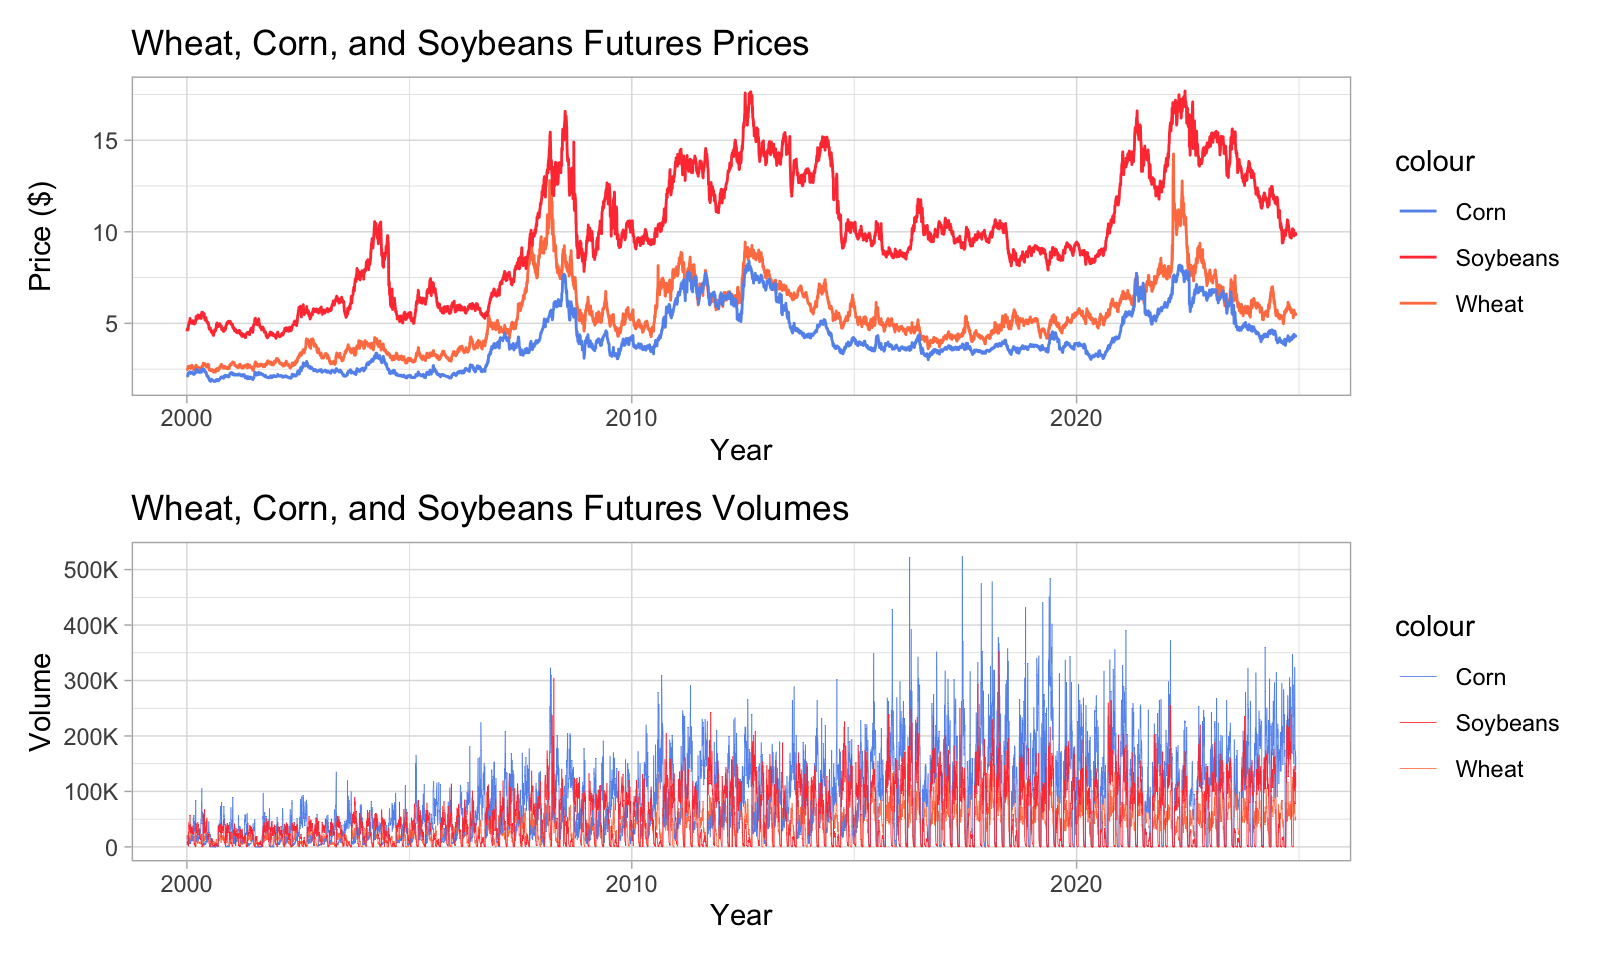
\includegraphics[width=0.85\textwidth]{figures/image13.png}

\textbf{Figure 1.} Prices and Trading Volumes of Wheat, Corn, and Soybeans Futures Contract
\newline
(January 2000 -- December 2024)
\end{center}
\bigskip

\begin{center}
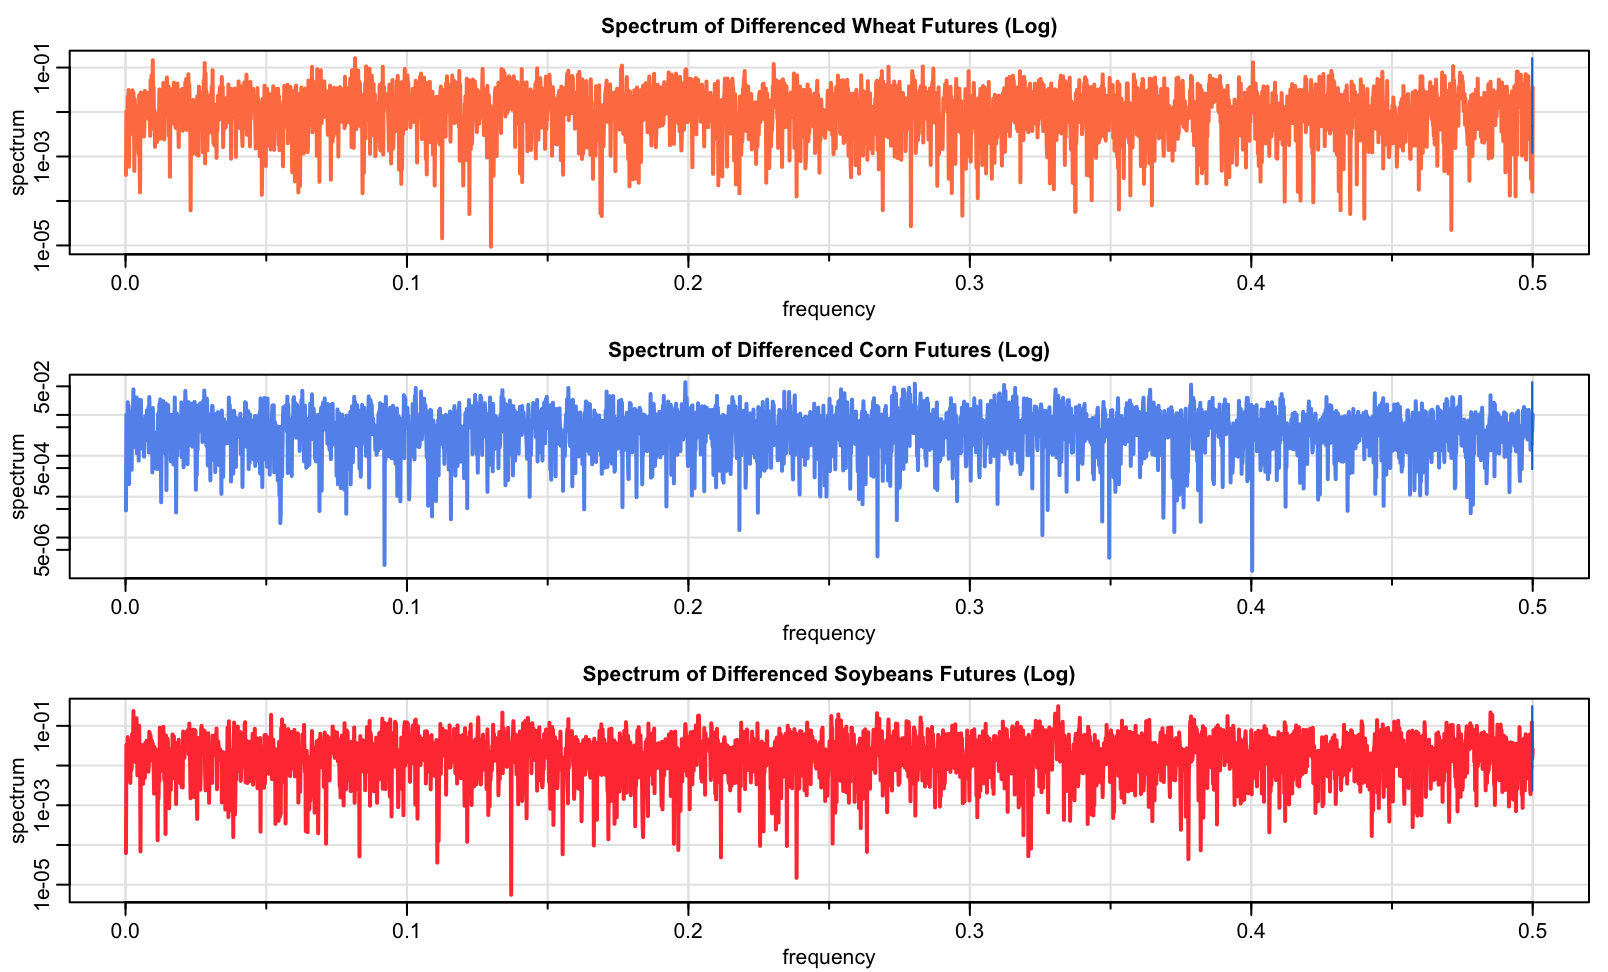
\includegraphics[width=0.85\textwidth]{figures/image17.png}

\textbf{Figure 2.} a. Spectrums of Differenced Wheat, Corn, and Soybeans Futures Prices
\end{center}
\bigskip

\begin{center}
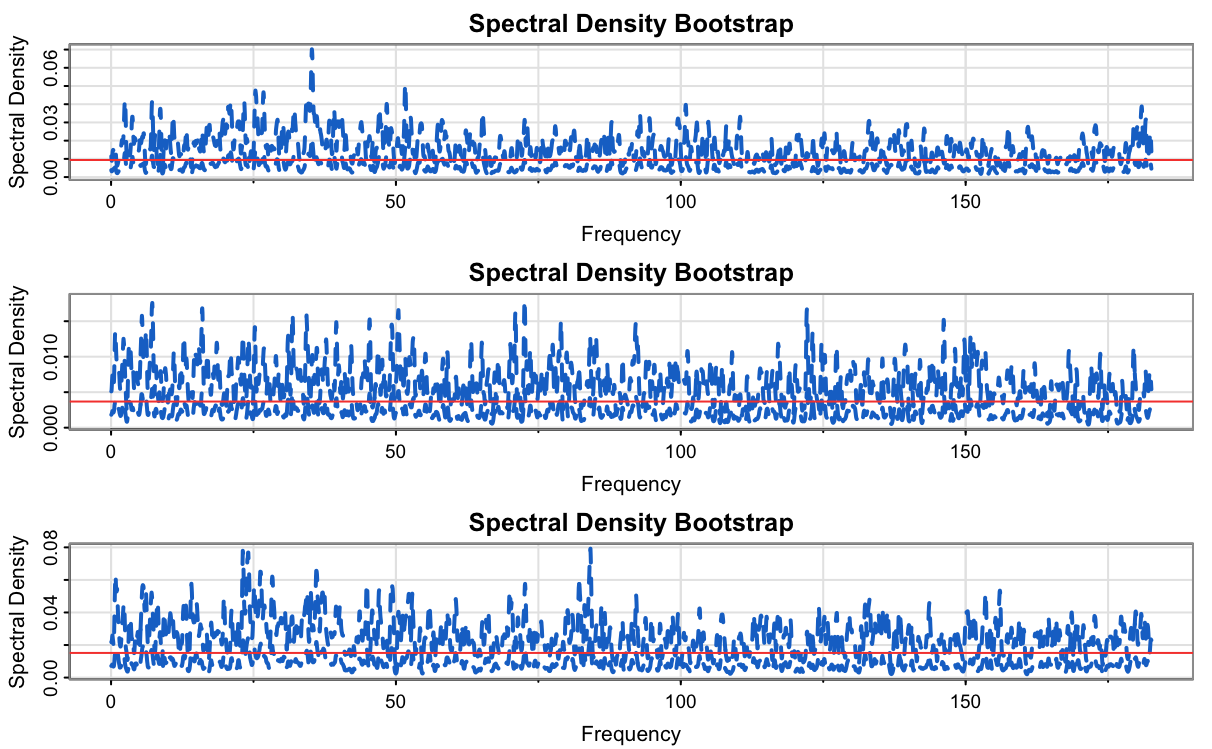
\includegraphics[width=0.9\textwidth]{figures/image27.png}

\textbf{Figure 2.} b. Spectral Density Bootstrap of Differenced Wheat, Corn, and Soybeans Futures Prices
\end{center}
\bigskip

\begin{center}
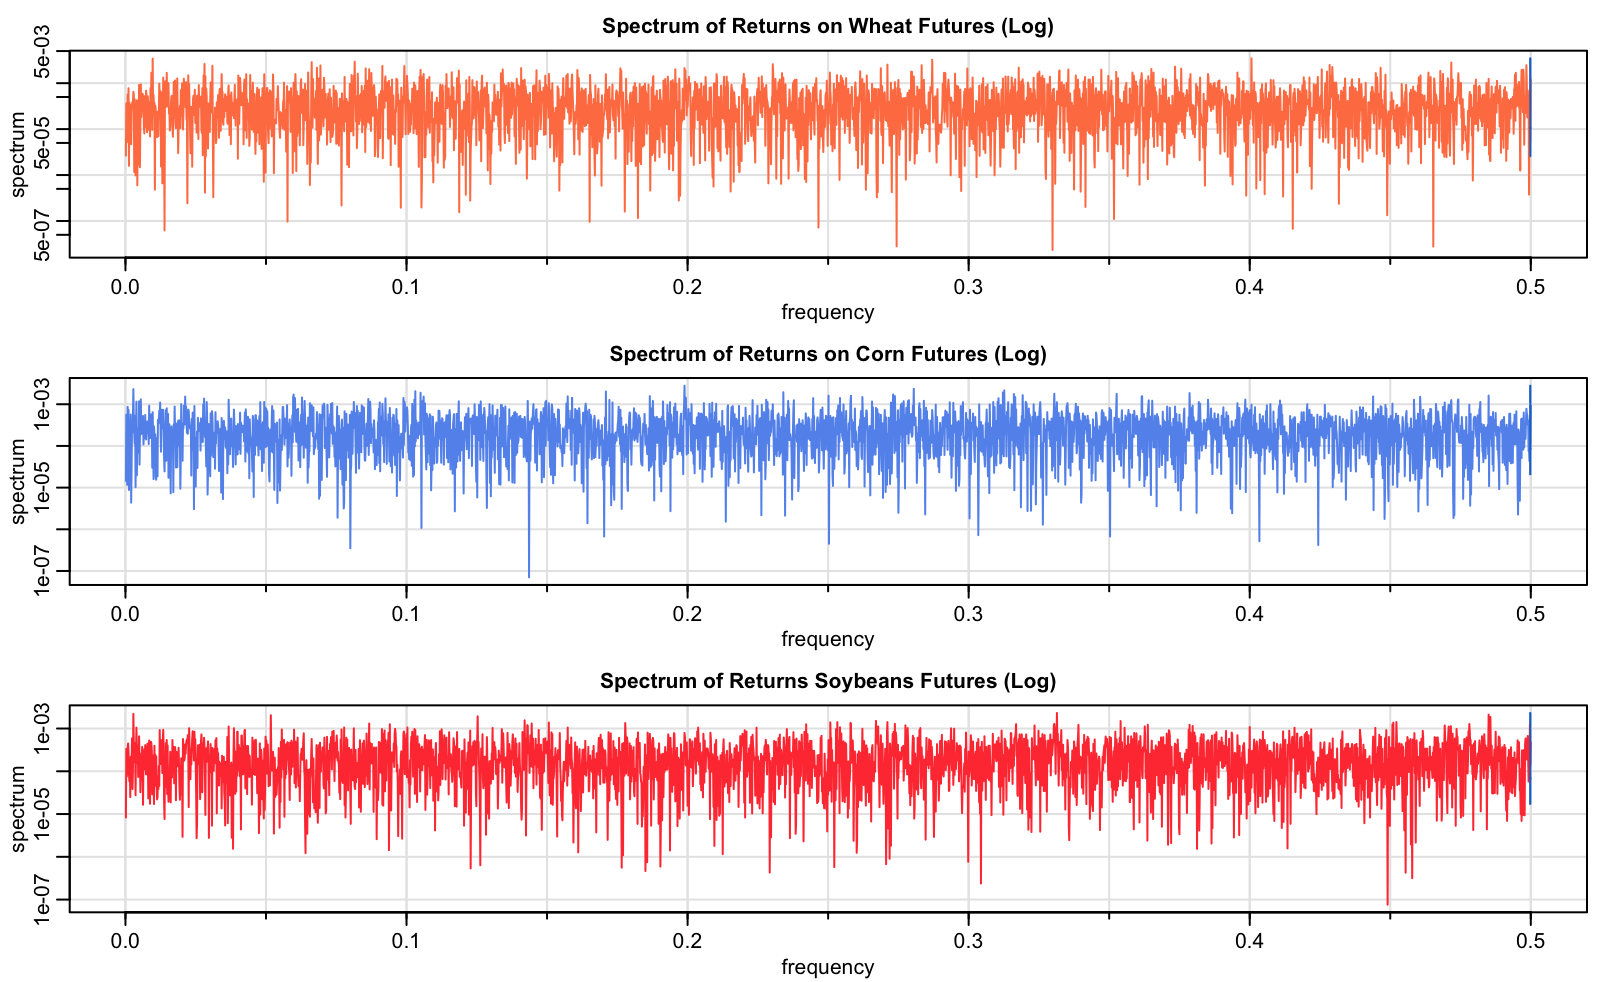
\includegraphics[width=0.9\textwidth]{figures/image40.png}

\textbf{Figure 2.} c. Spectrums of Returns on Wheat, Corn, and Soybeans Futures
\end{center}
\bigskip

\begin{center}
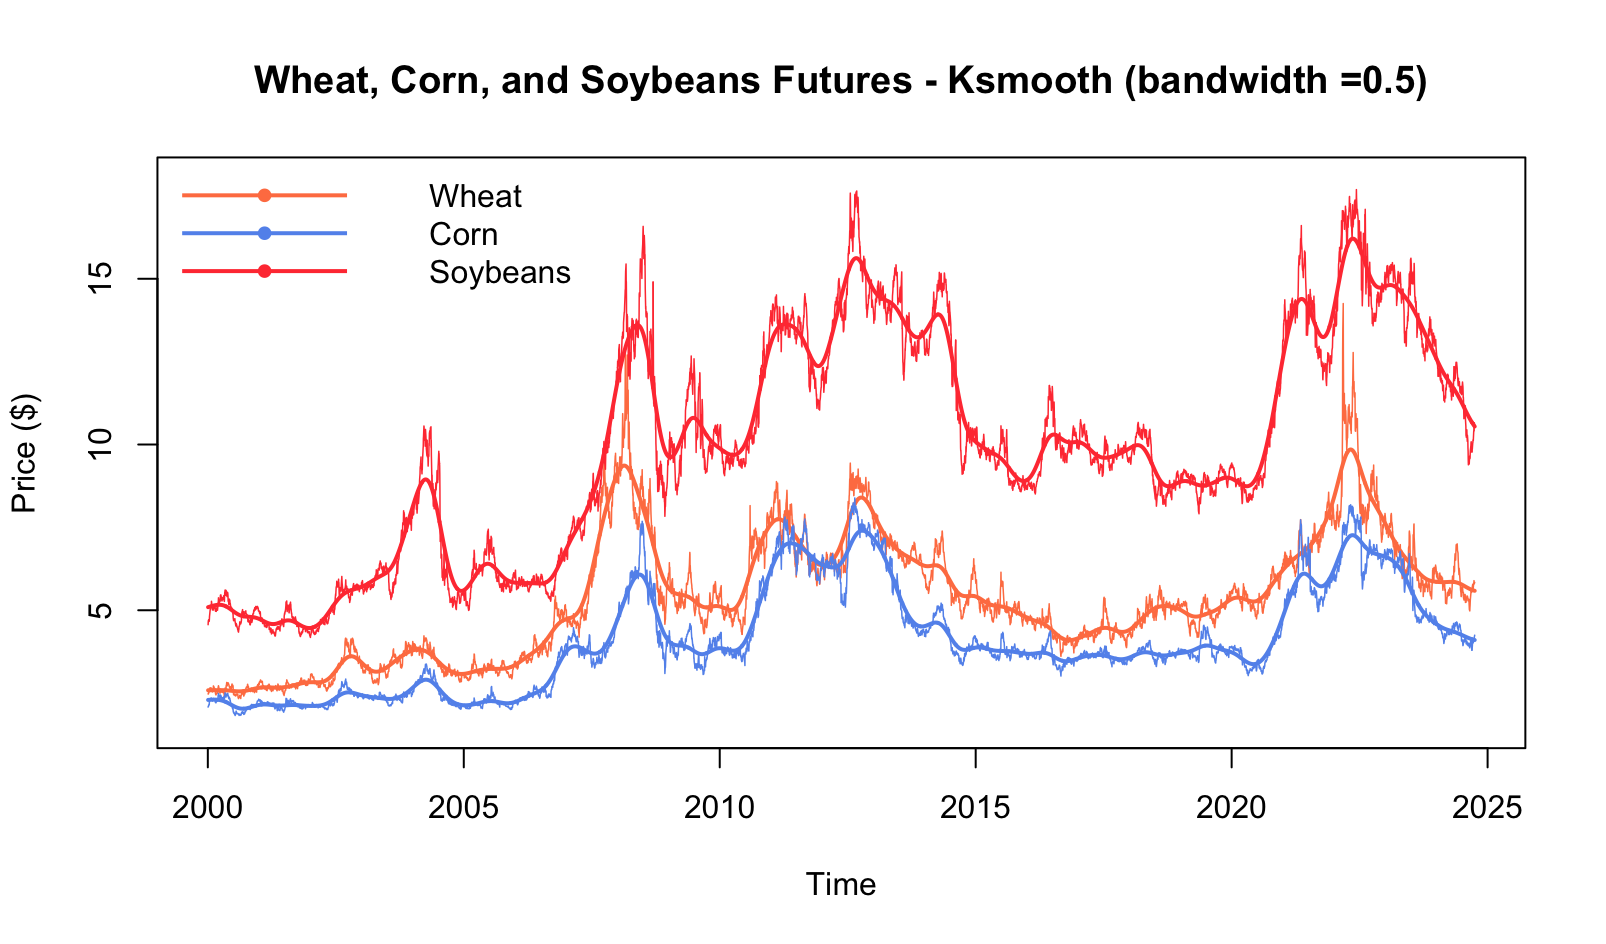
\includegraphics[width=0.85\textwidth]{figures/image39.png}\\[0.5em]
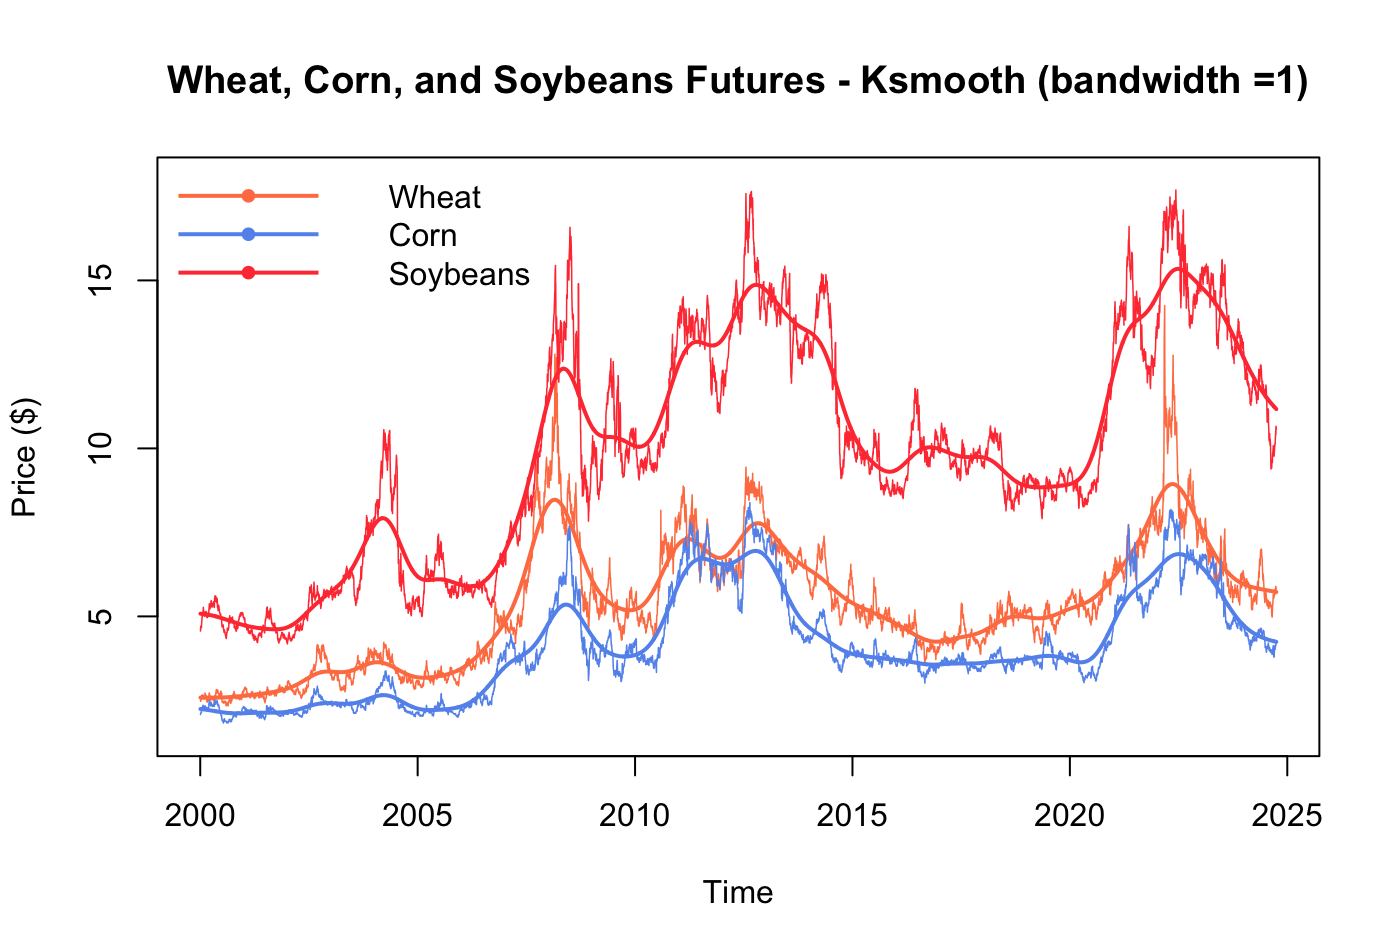
\includegraphics[width=\textwidth]{figures/image18.png}

\textbf{Figure 3.} Closing Prices of Wheat, Corn, and Soybeans Futures Contract with Smoothers (January 2000 -- December 2024)
\end{center}
\bigskip

\begin{center}
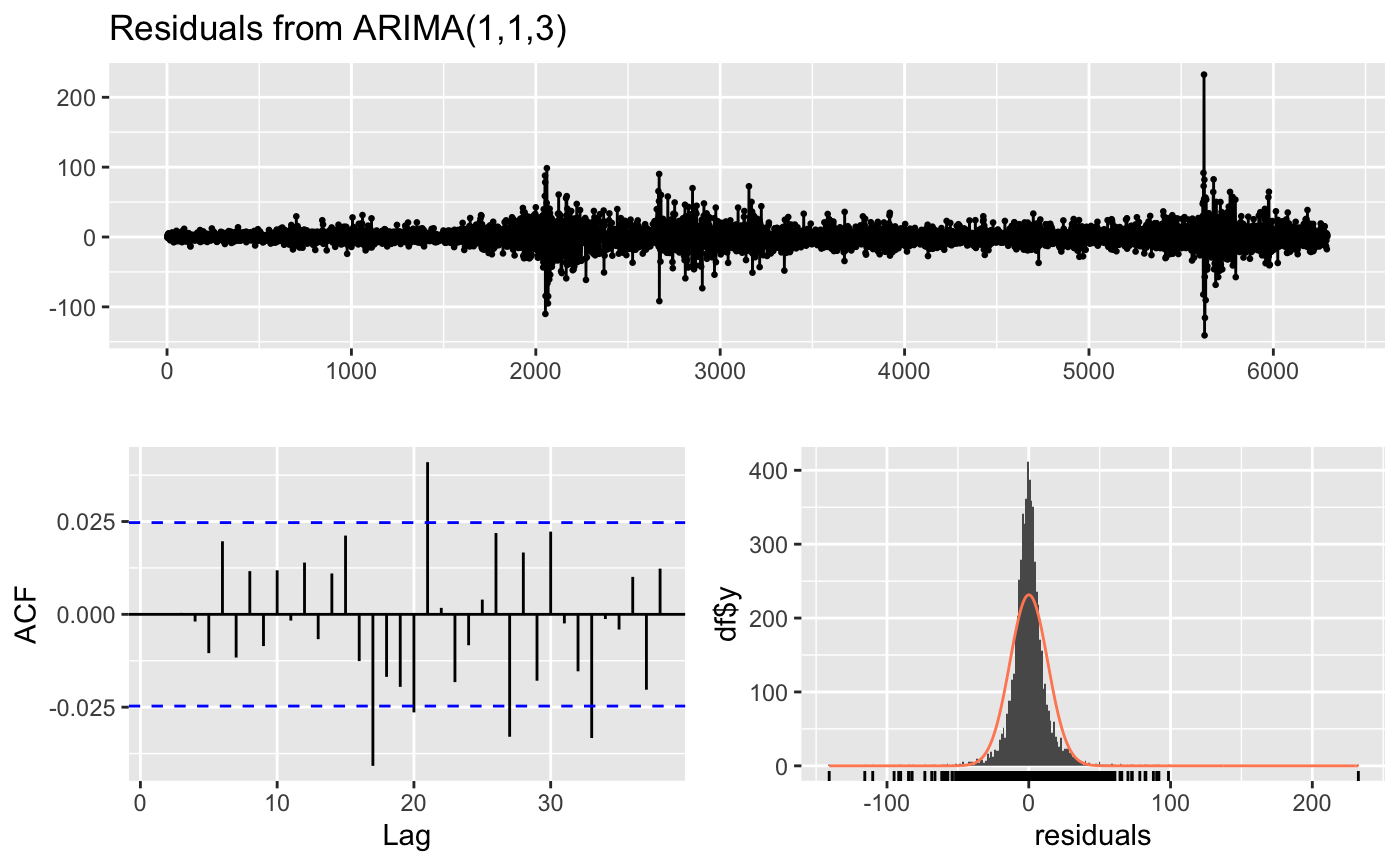
\includegraphics[width=0.85\textwidth]{figures/image11.png}\\[0.5em]
\begin{minipage}{0.48\textwidth}\centering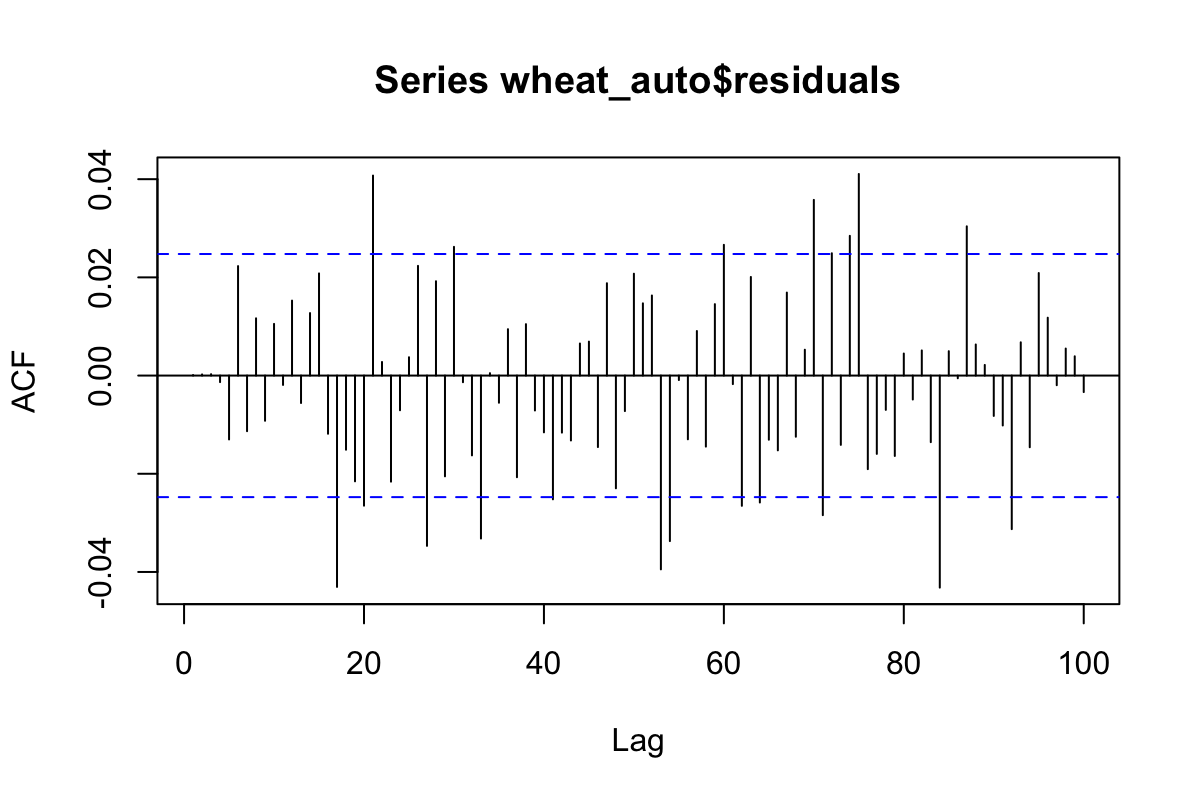
\includegraphics[width=\textwidth]{figures/image34.png}\end{minipage}
\begin{minipage}{0.48\textwidth}\centering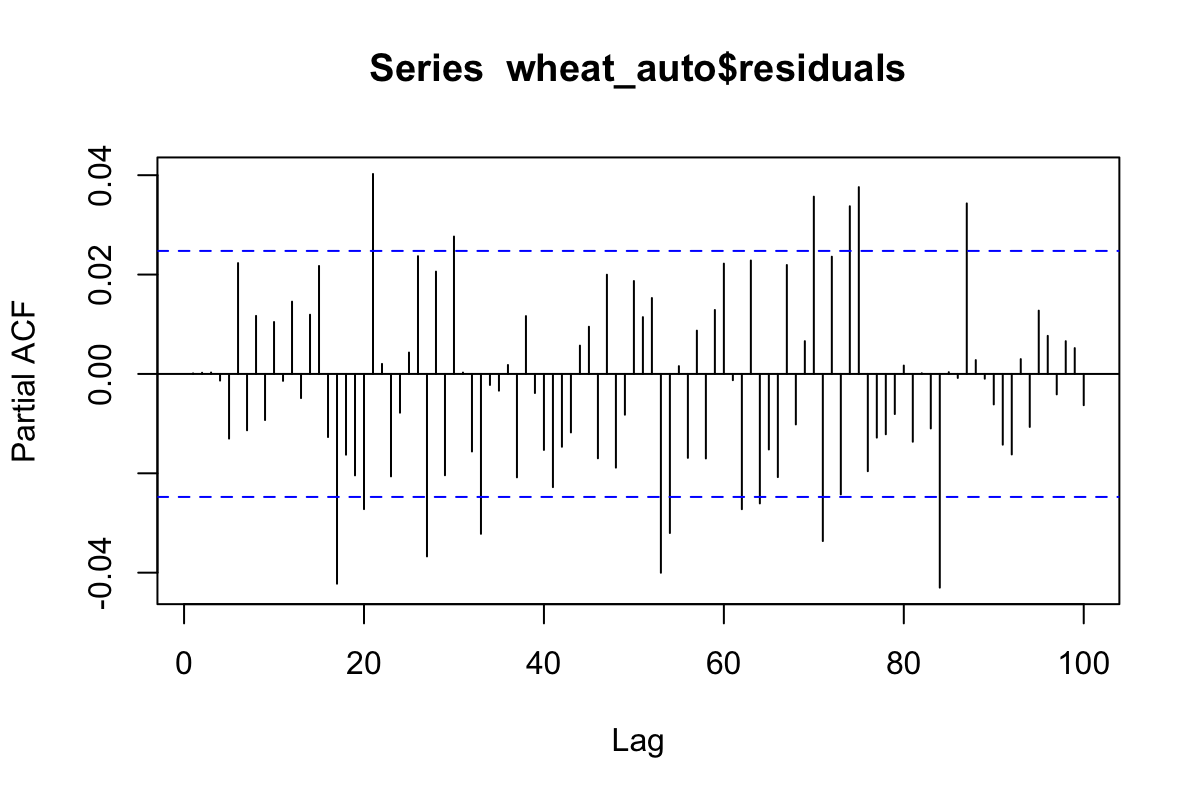
\includegraphics[width=\textwidth]{figures/image9.png}\end{minipage}\\[0.5em]
\begin{minipage}{0.48\textwidth}\centering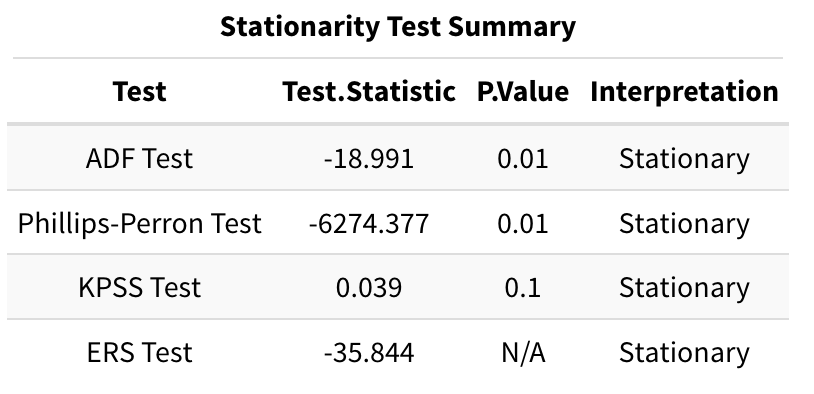
\includegraphics[width=\textwidth]{figures/image43.png}\end{minipage}
\begin{minipage}{0.48\textwidth}\centering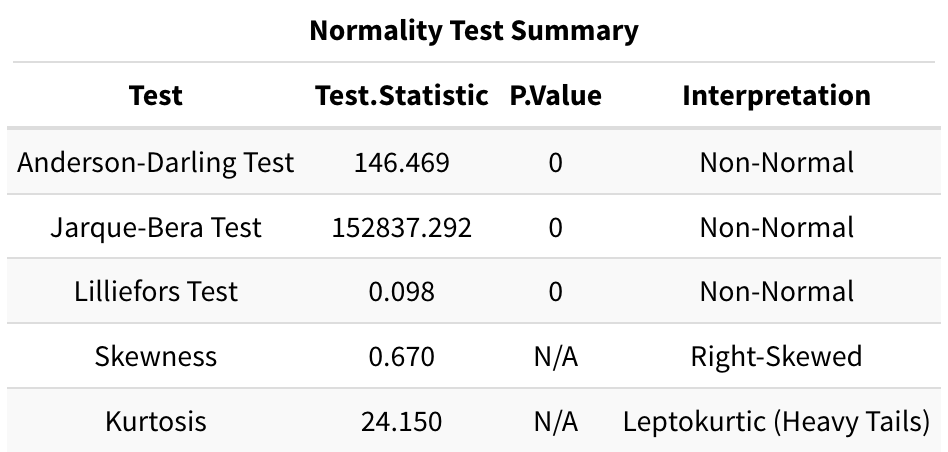
\includegraphics[width=\textwidth]{figures/image20.png}\end{minipage}

\textbf{Figure 4.} ARIMA(1,1,3) model fitted on US daily wheat futures prices. The model's residuals are stationary, but not independent and not normal, suggesting interpreting forecasts with caution.
\end{center}
\bigskip

\begin{center}
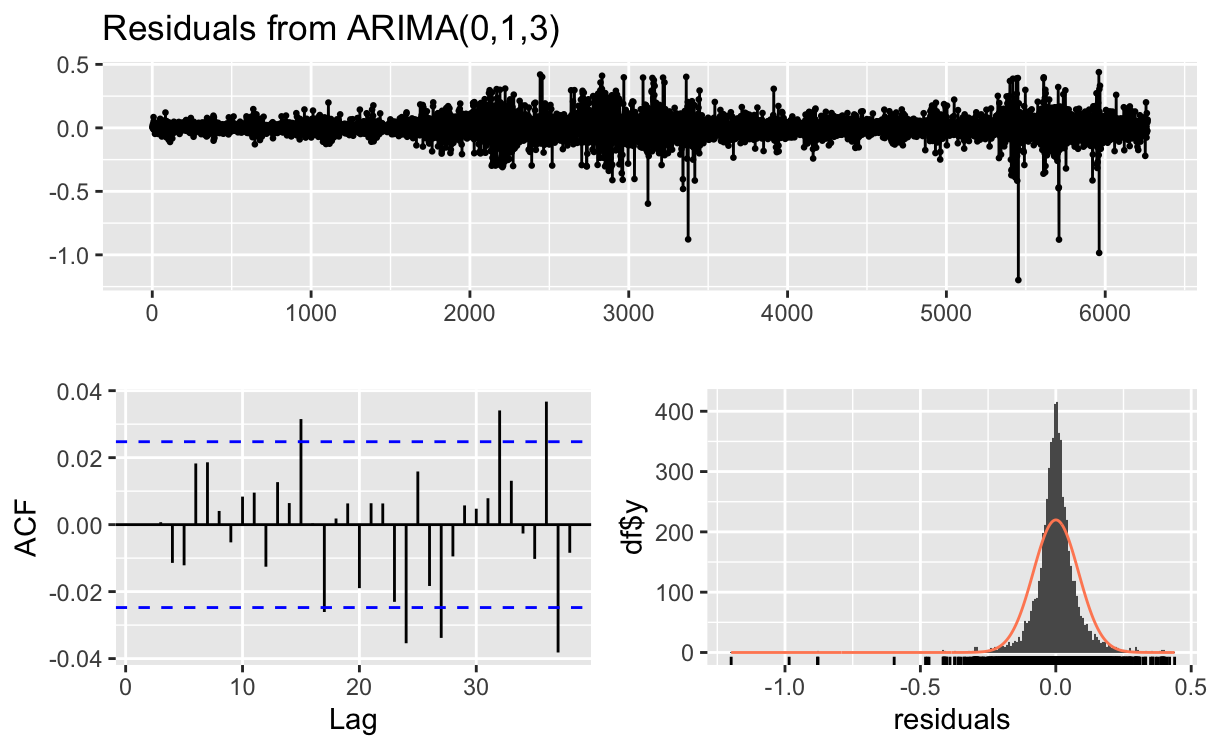
\includegraphics[width=0.85\textwidth]{figures/image22.png}\\[0.5em]
\begin{minipage}{0.48\textwidth}\centering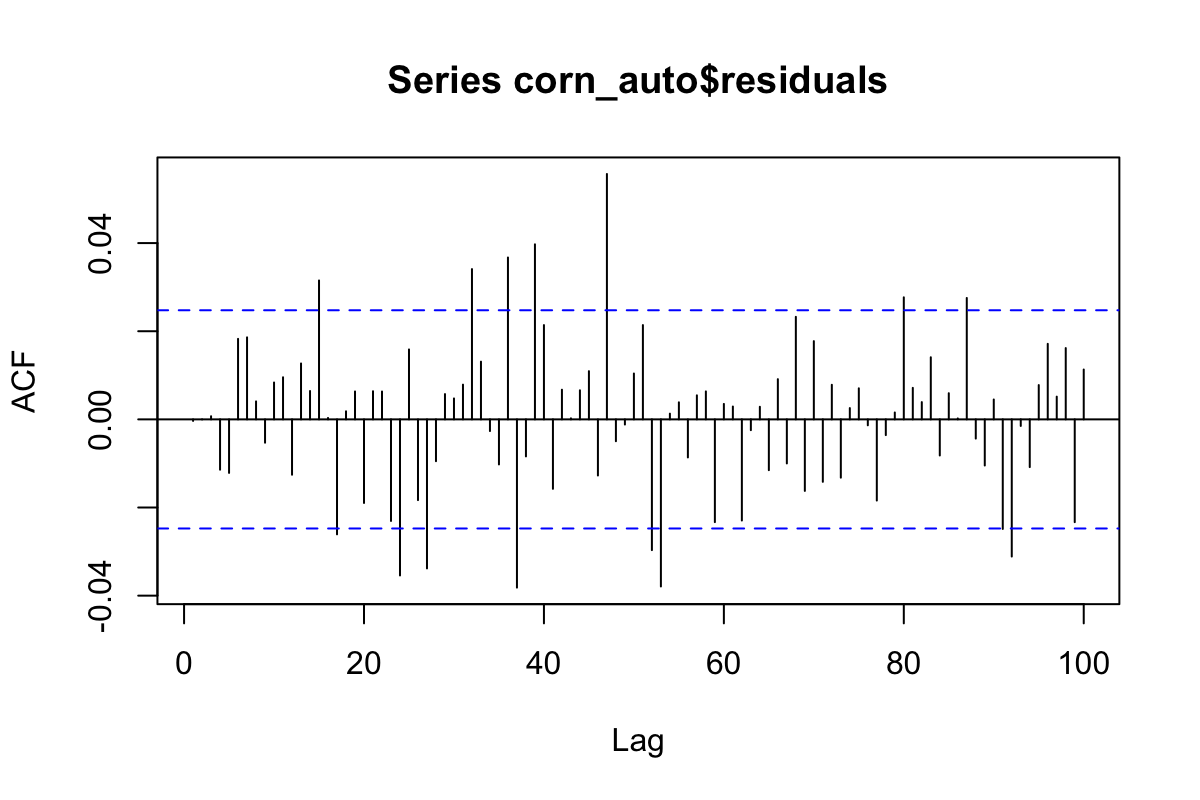
\includegraphics[width=\textwidth]{figures/image29.png}\end{minipage}
\begin{minipage}{0.48\textwidth}\centering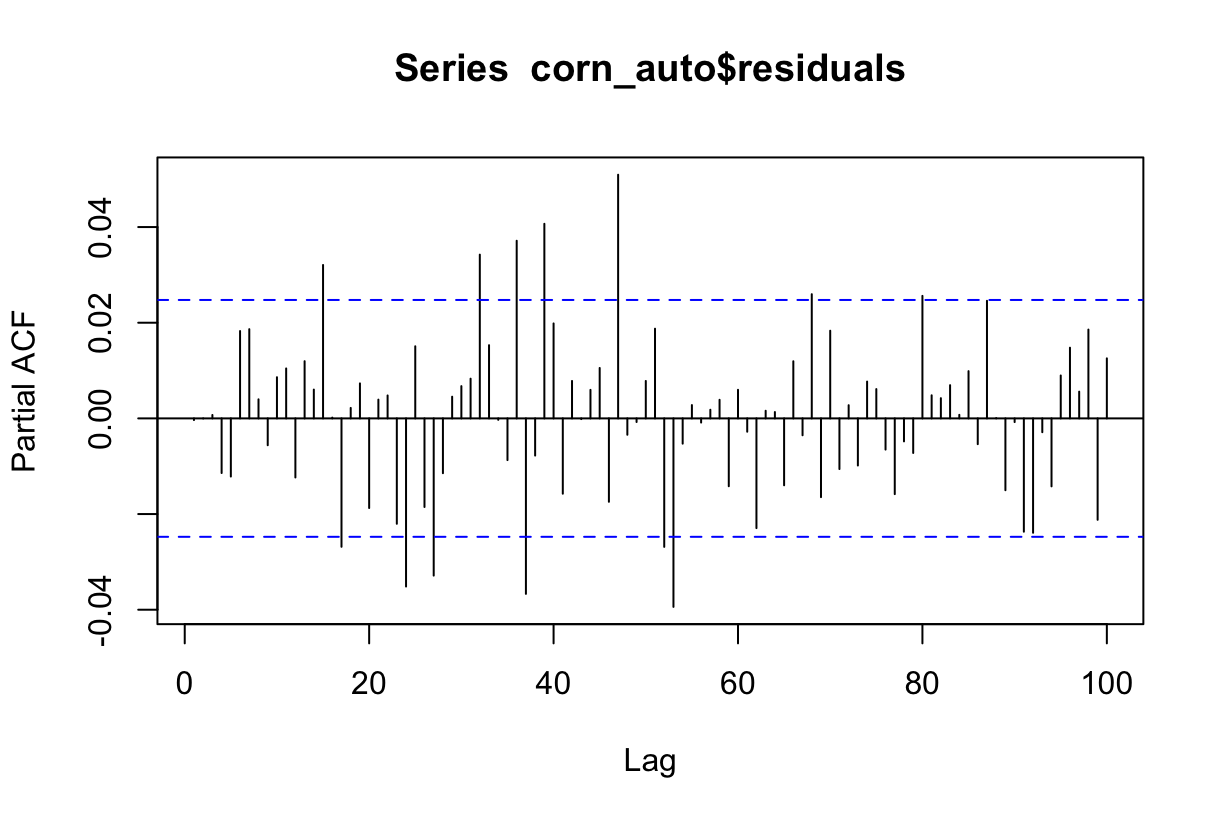
\includegraphics[width=\textwidth]{figures/image32.png}\end{minipage}\\[0.5em]
\begin{minipage}{0.48\textwidth}\centering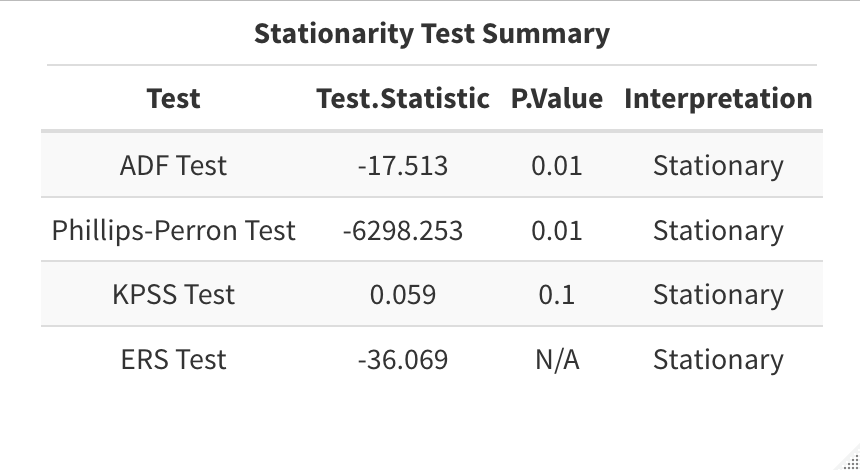
\includegraphics[width=\textwidth]{figures/image16.png}\end{minipage}
\begin{minipage}{0.48\textwidth}\centering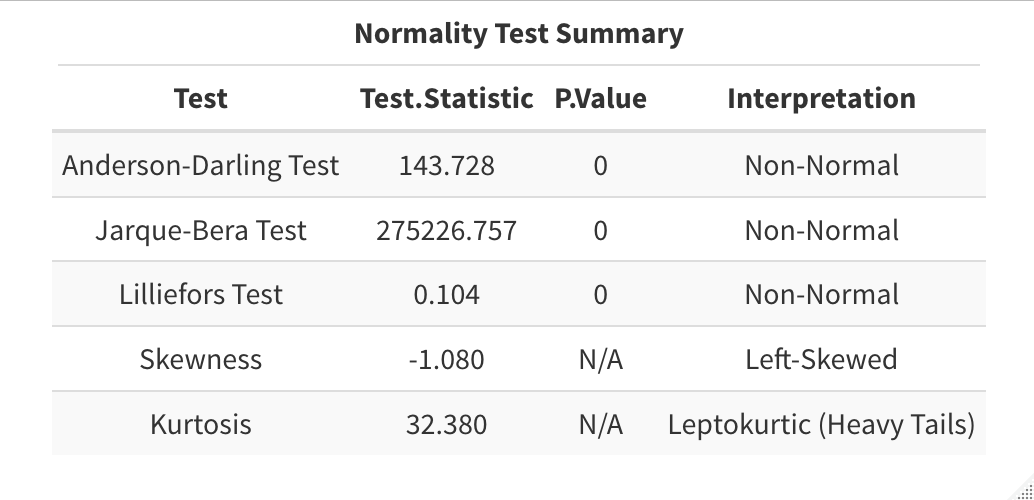
\includegraphics[width=\textwidth]{figures/image21.png}\end{minipage}

\textbf{Figure 5.} ARIMA(0,1,3) model fitted on US daily corn futures prices. The model's residuals are stationary, but not independent and not normal, suggesting interpreting forecasts with caution.
\end{center}
\bigskip

\begin{center}
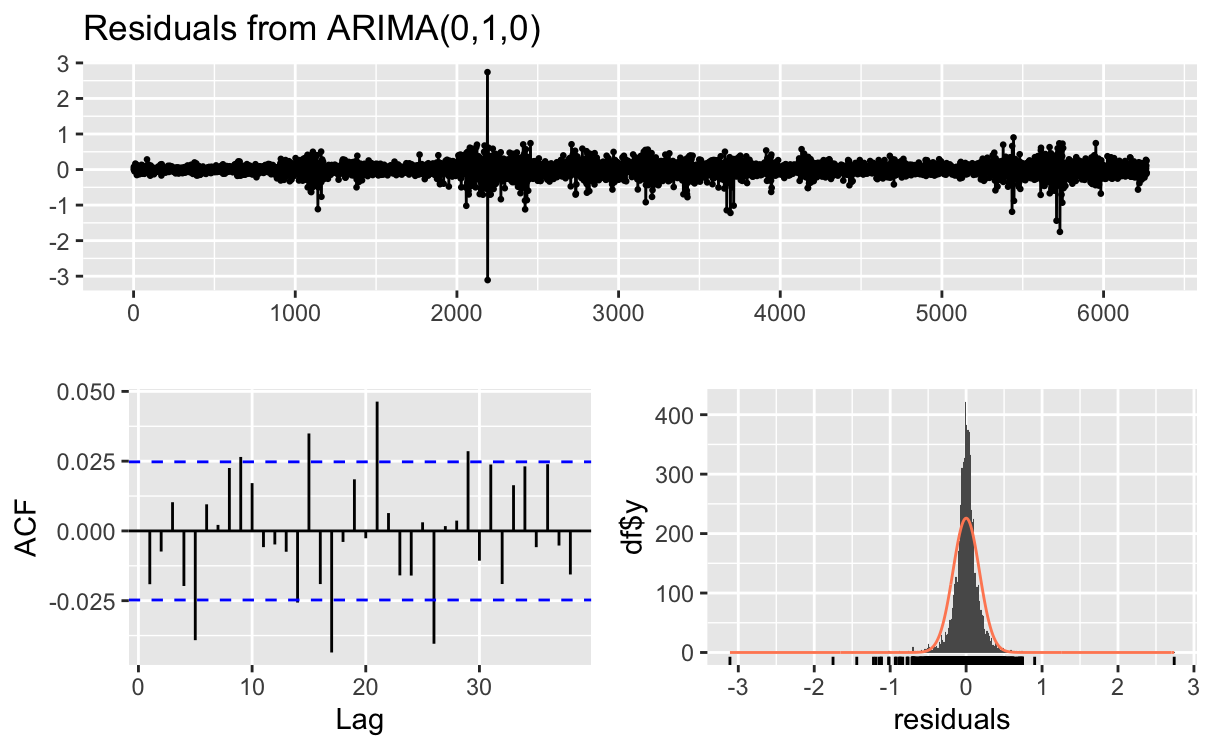
\includegraphics[width=0.85\textwidth]{figures/image28.png}\\[0.5em]
\begin{minipage}{0.48\textwidth}\centering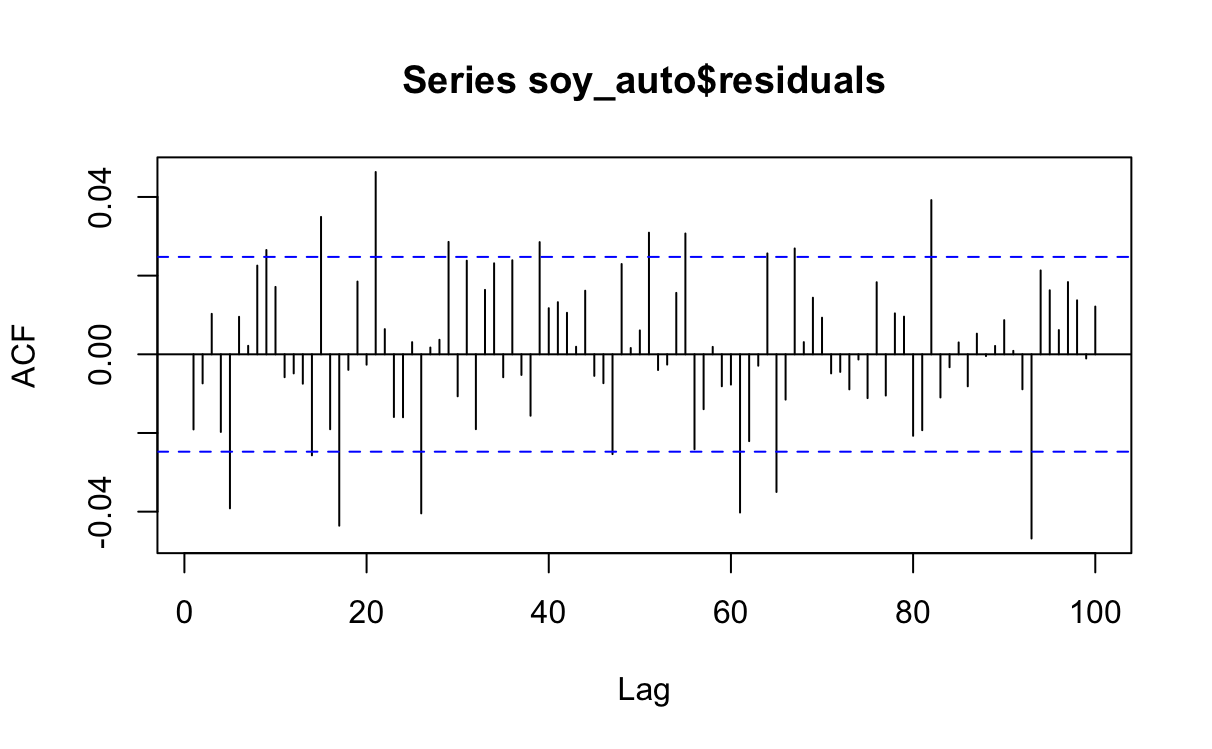
\includegraphics[width=\textwidth]{figures/image44.png}\end{minipage}
\begin{minipage}{0.48\textwidth}\centering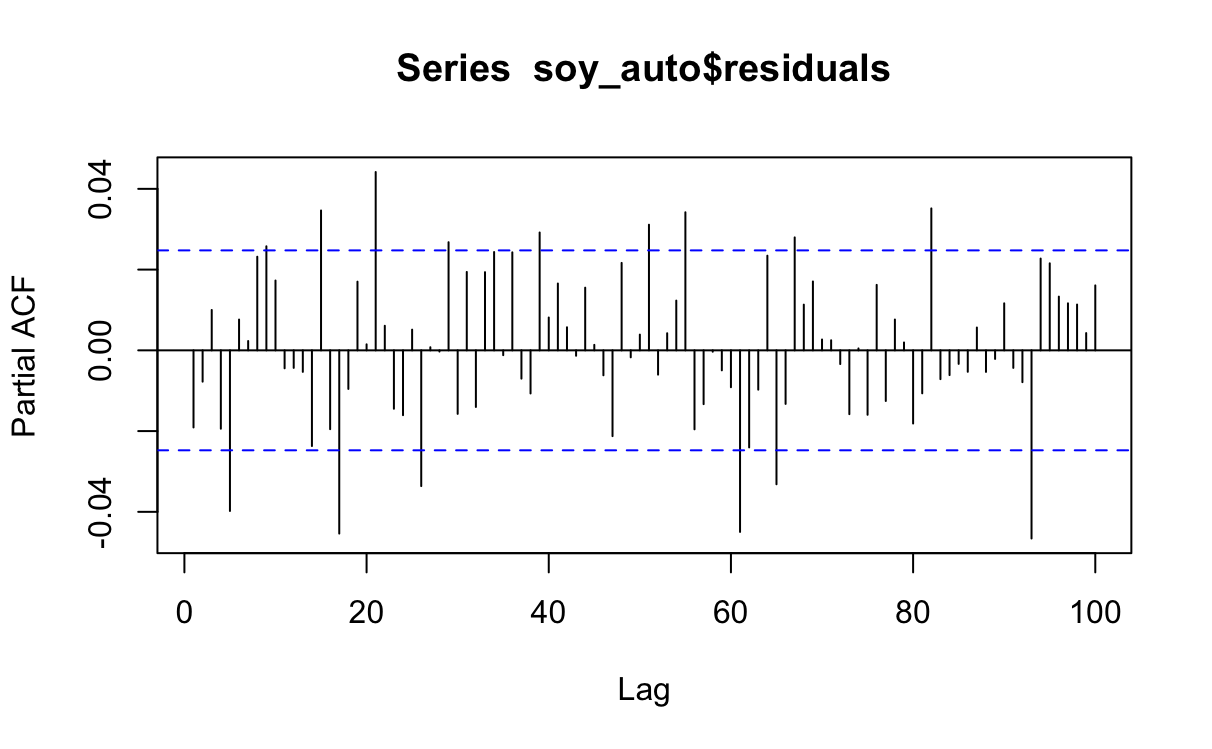
\includegraphics[width=\textwidth]{figures/image2.png}\end{minipage}\\[0.5em]
\begin{minipage}{0.48\textwidth}\centering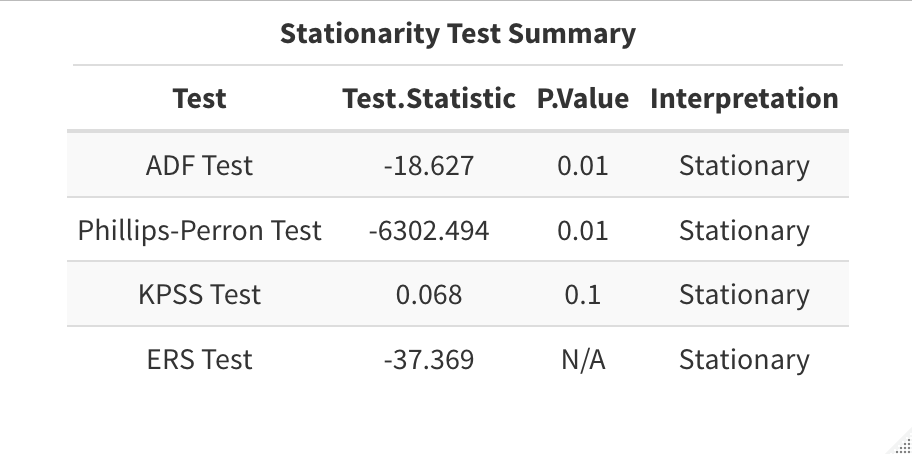
\includegraphics[width=\textwidth]{figures/image5.png}\end{minipage}
\begin{minipage}{0.48\textwidth}\centering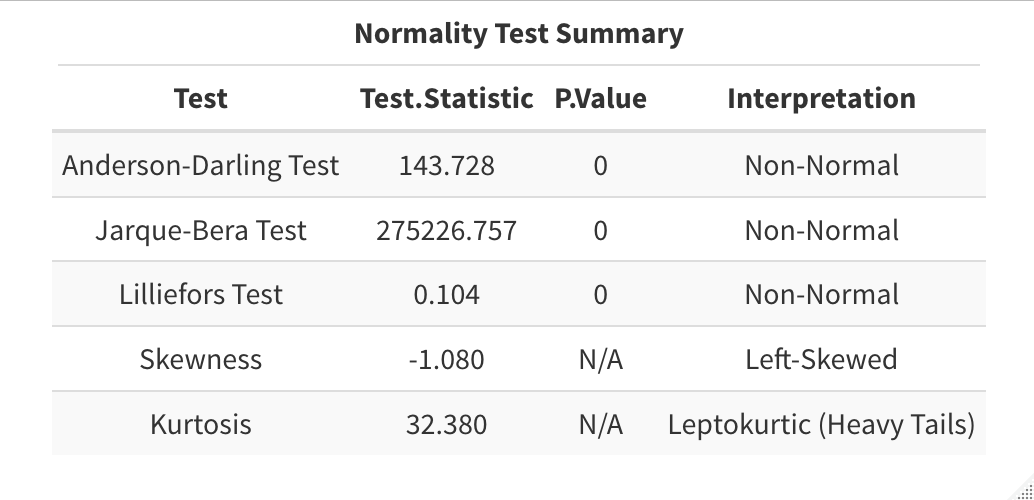
\includegraphics[width=\textwidth]{figures/image21.png}\end{minipage}

\textbf{Figure 6.} ARIMA(0,1,0) model fitted on US daily soybeans futures prices. The model's residuals are stationary, but not independent and not normal, suggesting interpreting forecasts with caution.
\end{center}
\bigskip

\begin{center}
\begin{minipage}{0.48\textwidth}\centering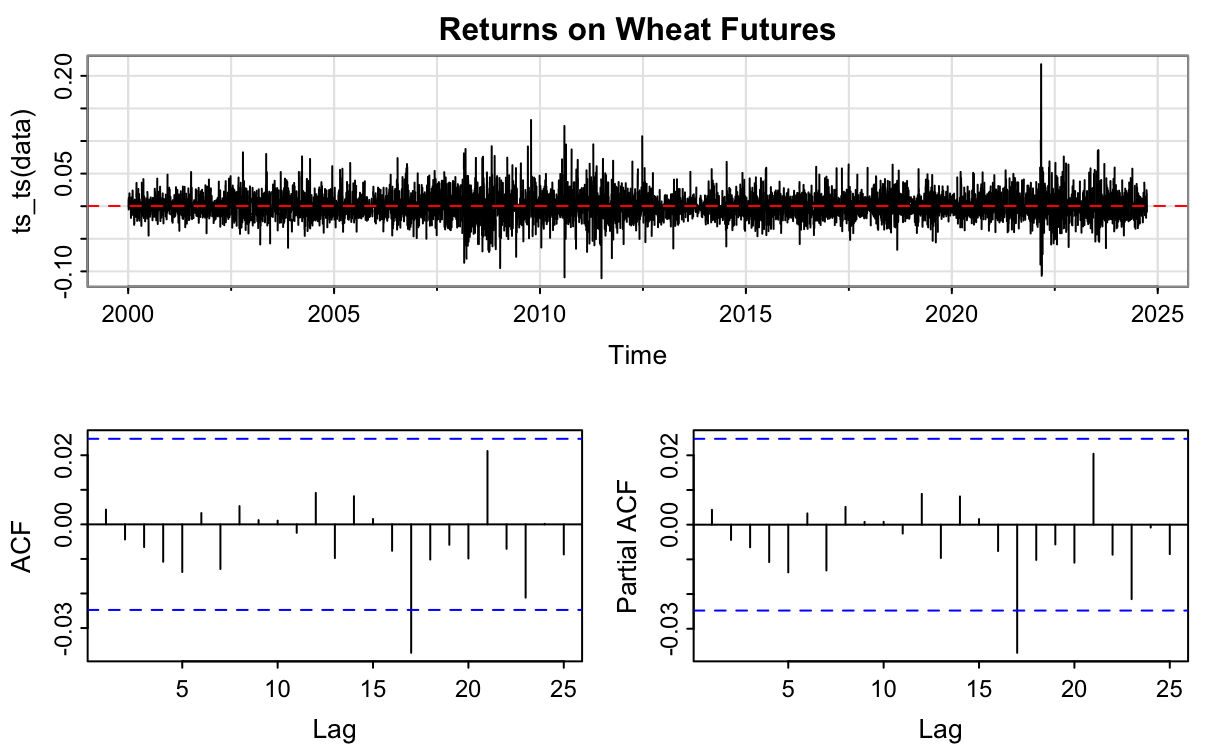
\includegraphics[width=\textwidth]{figures/image7.png}\end{minipage}
\begin{minipage}{0.48\textwidth}\centering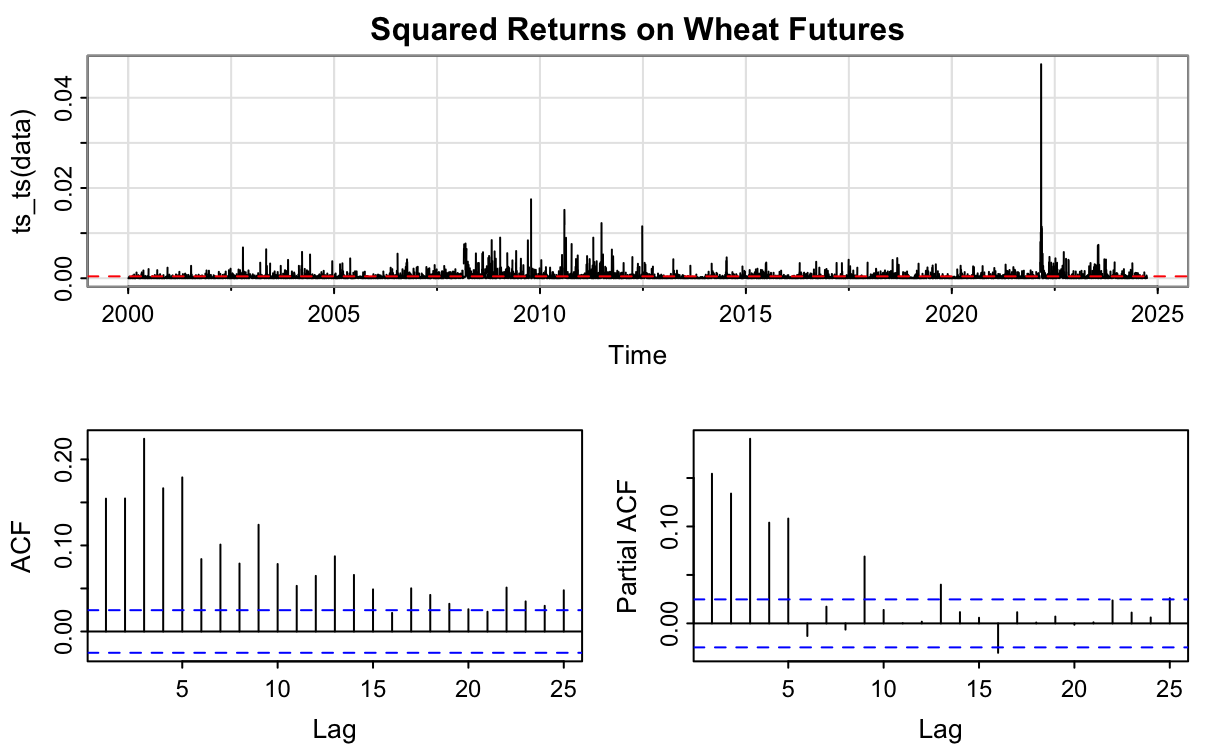
\includegraphics[width=\textwidth]{figures/image38.png}\end{minipage}\\[0.5em]
\begin{minipage}{0.48\textwidth}\centering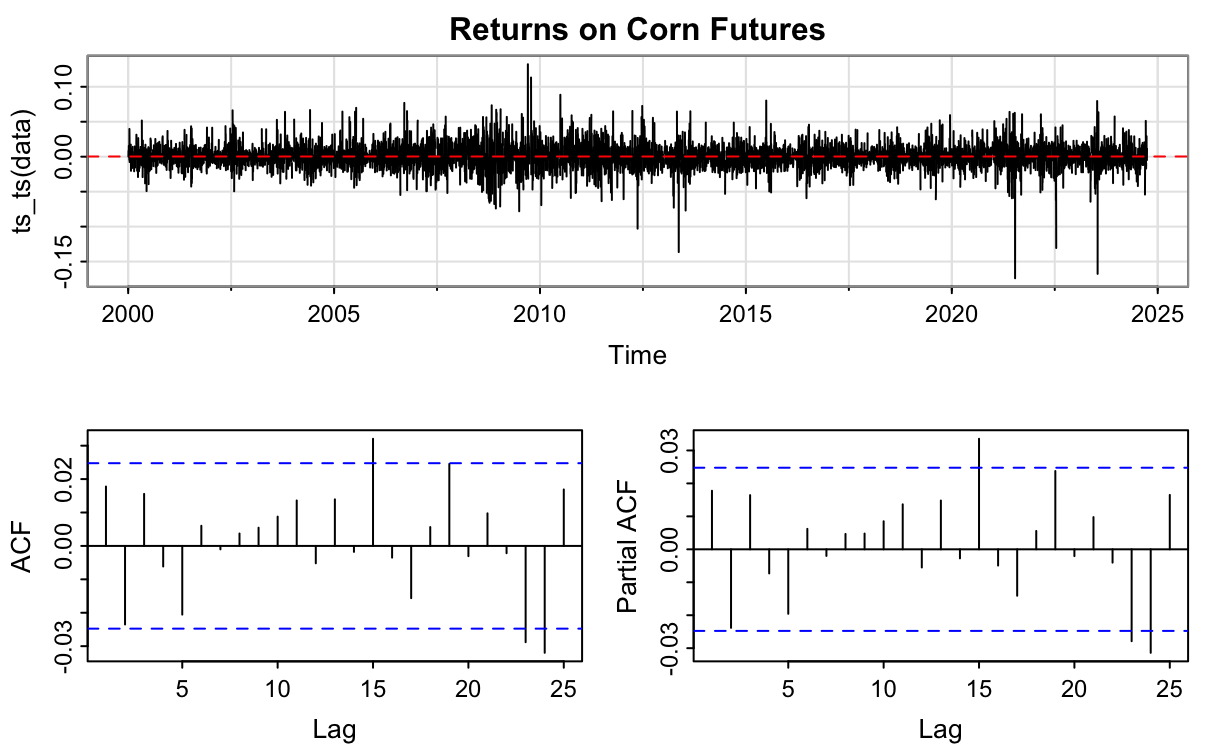
\includegraphics[width=\textwidth]{figures/image14.png}\end{minipage}
\begin{minipage}{0.48\textwidth}\centering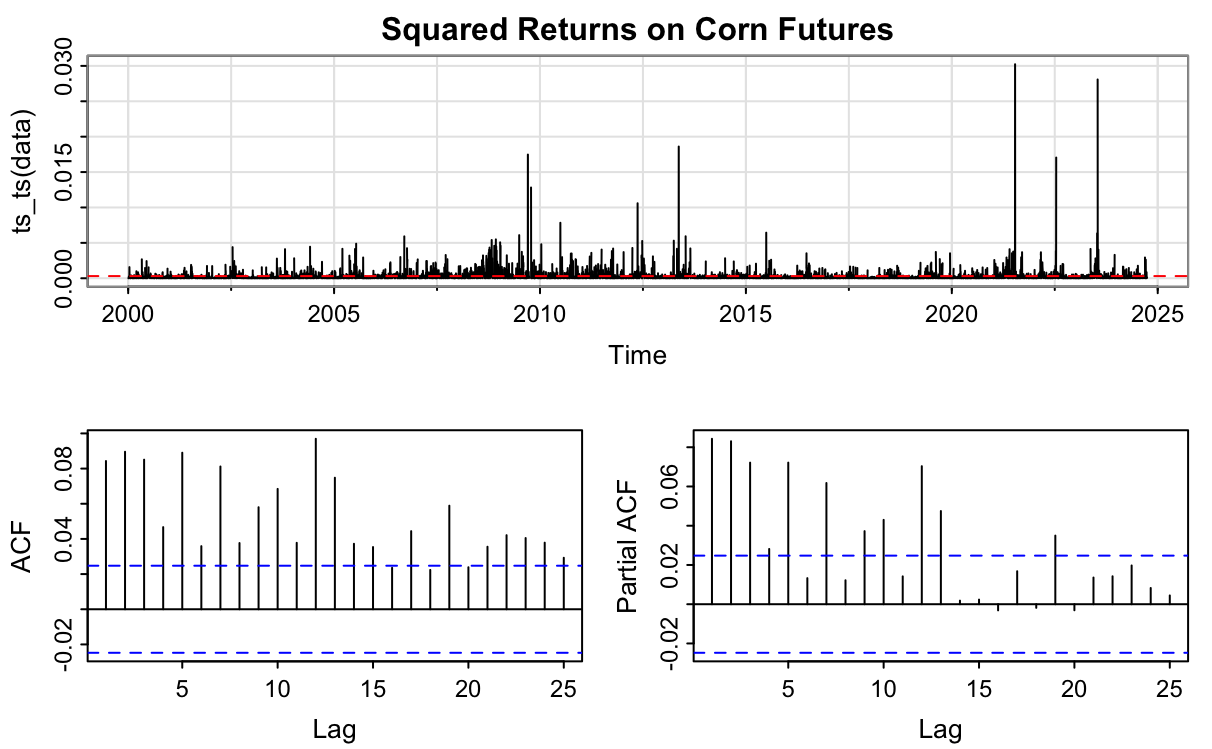
\includegraphics[width=\textwidth]{figures/image10.png}\end{minipage}\\[0.5em]
\begin{minipage}{0.48\textwidth}\centering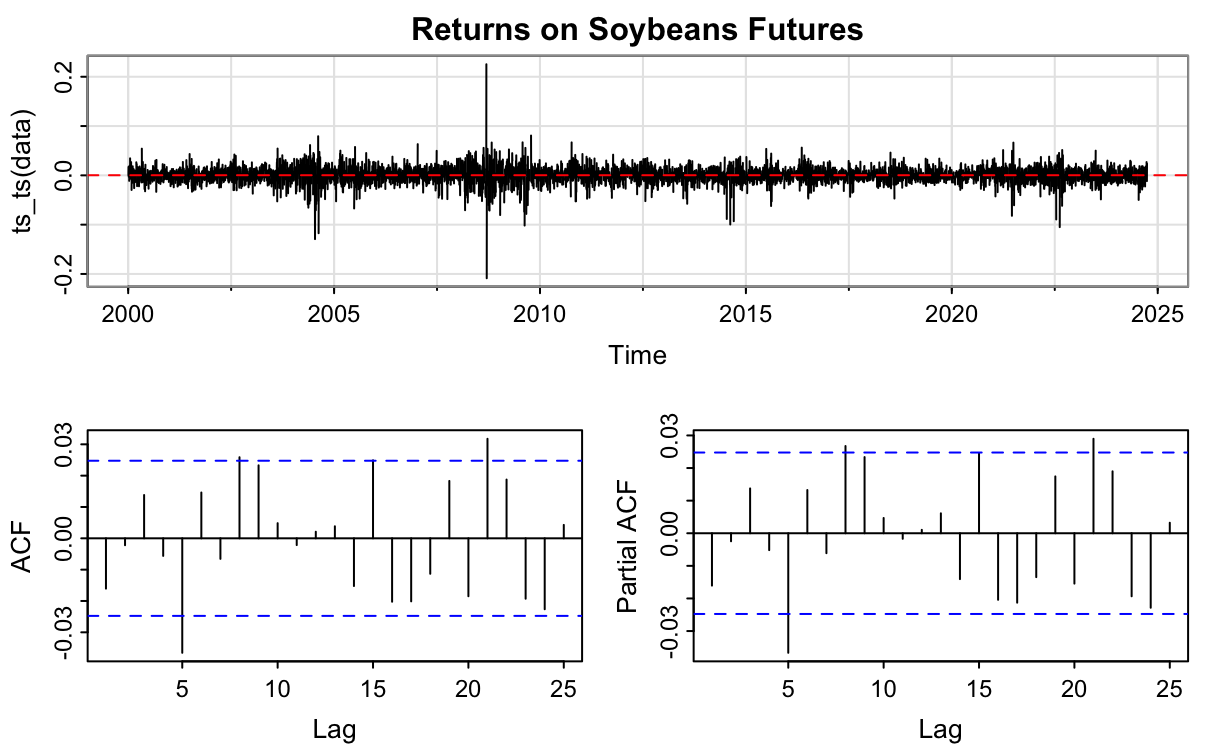
\includegraphics[width=\textwidth]{figures/image30.png}\end{minipage}
\begin{minipage}{0.48\textwidth}\centering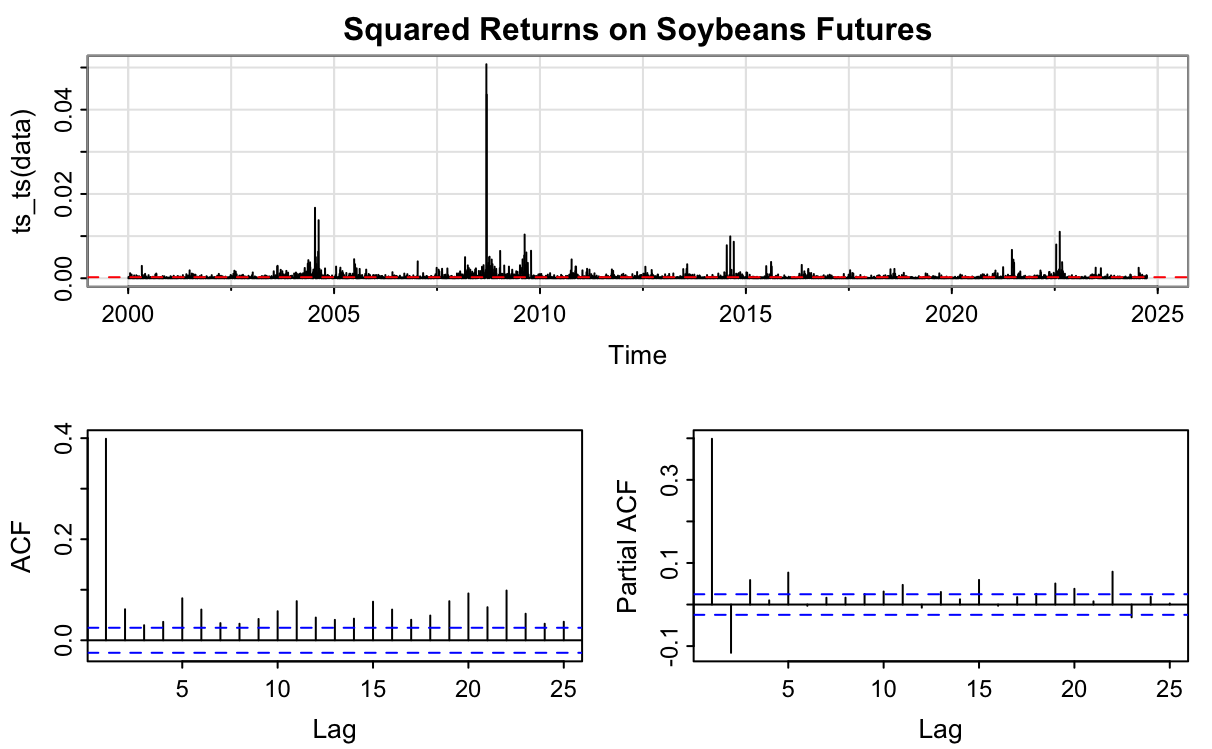
\includegraphics[width=\textwidth]{figures/image42.png}\end{minipage}

\textbf{Figure 7.} Analysis of Return and Squared Returns Series of Wheat, Corn, and Soybeans Futures
\end{center}
\skip

\begin{center}
\begin{minipage}{0.48\textwidth}\centering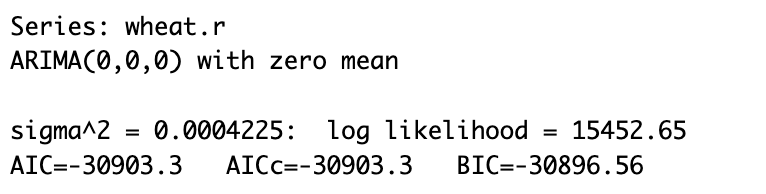
\includegraphics[width=\textwidth]{figures/image19.png}\end{minipage}
\begin{minipage}{0.48\textwidth}\centering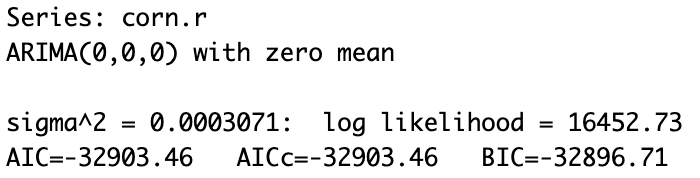
\includegraphics[width=\textwidth]{figures/image23.png}\end{minipage}\\[0.5em]
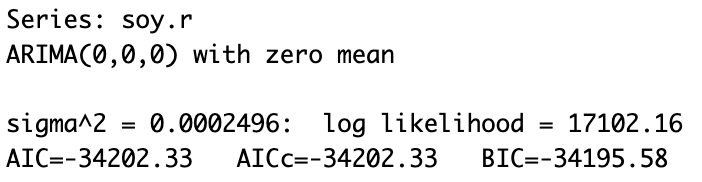
\includegraphics[width=0.65\textwidth]{figures/image37.png}

\textbf{Figure 8.} ARIMA models suggested by auto.arima() for the returns series of wheat, corn, and soybean futures
\end{center}
\bigskip

\begin{center}
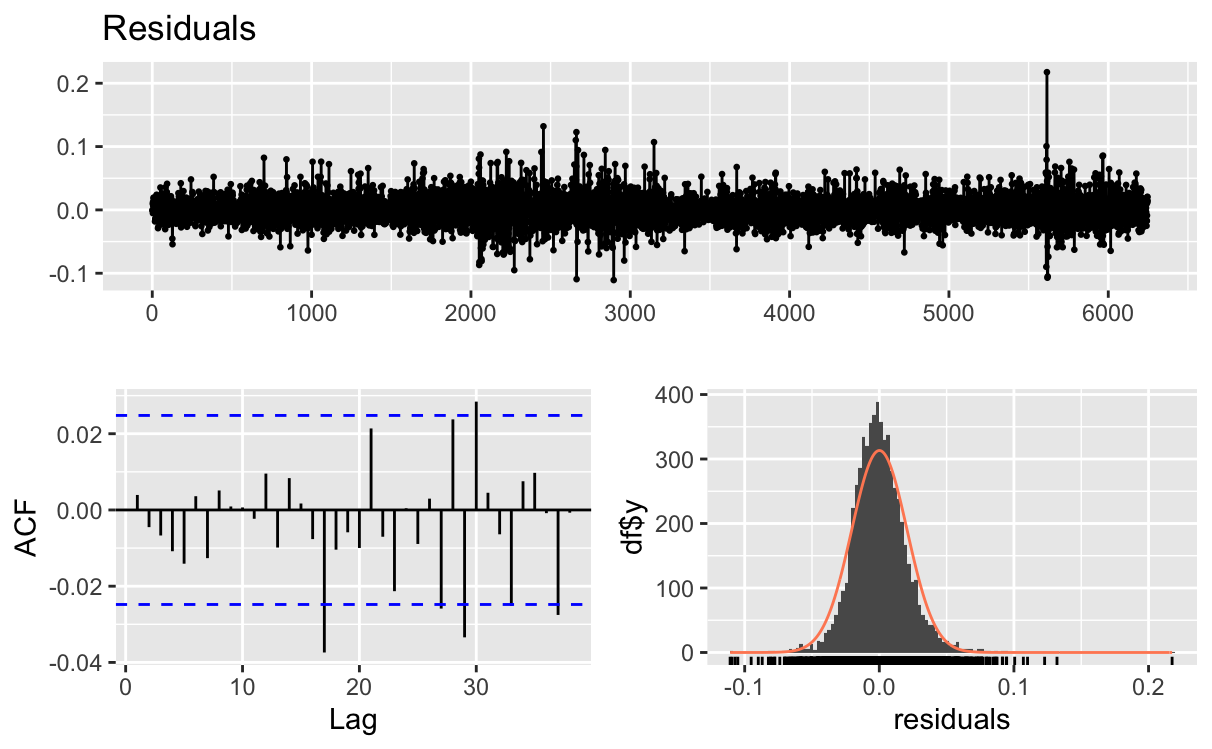
\includegraphics[width=0.85\textwidth]{figures/image41.png}\\[0.5em]
\begin{minipage}{0.48\textwidth}\centering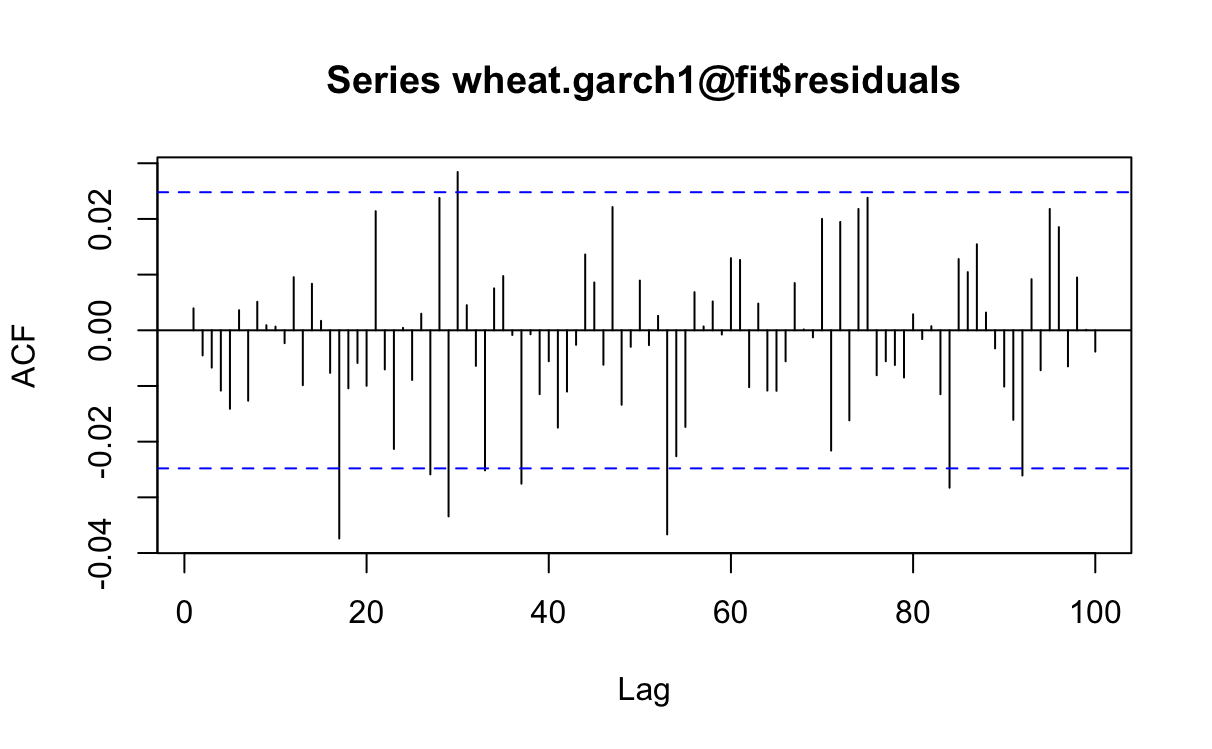
\includegraphics[width=\textwidth]{figures/image1.png}\end{minipage}
\begin{minipage}{0.48\textwidth}\centering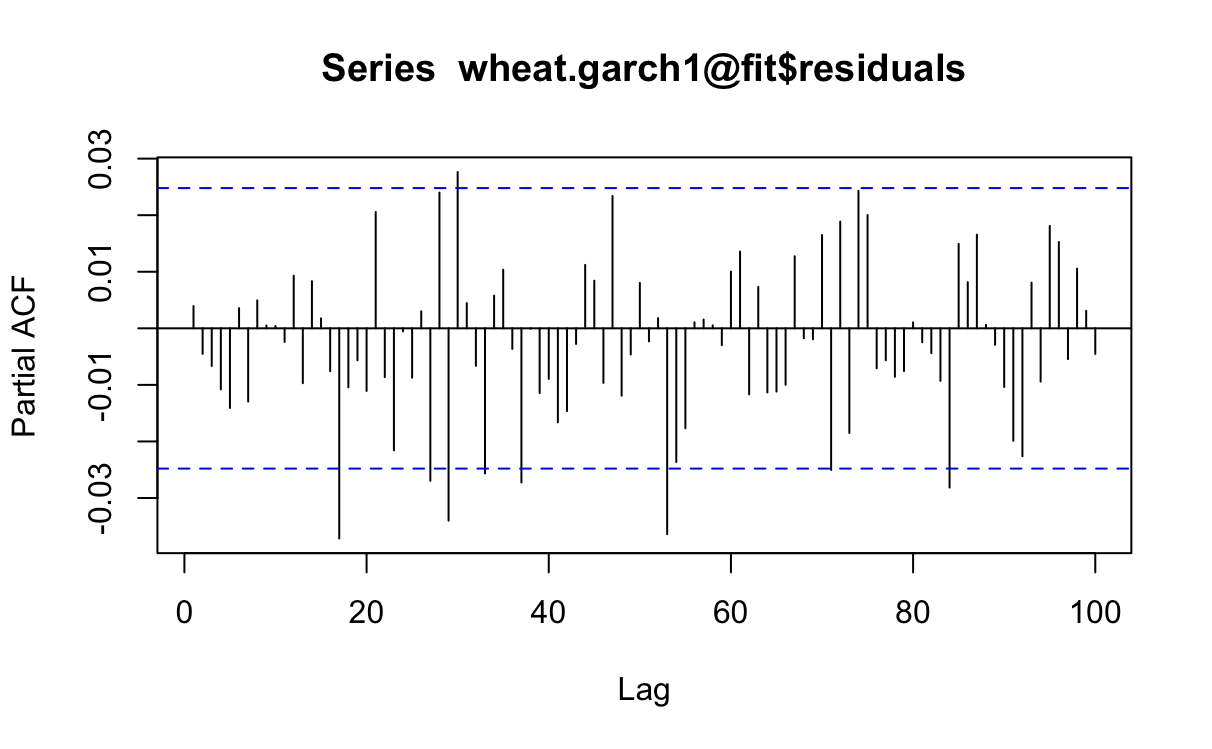
\includegraphics[width=\textwidth]{figures/image33.png}\end{minipage}

\textbf{Figure 9.} ARFIMA(0,0,0) + GARCH(1,1) with skewed Student-t distribution fitted on daily returns of US wheat futures prices. The model's residuals are stationary, independent, and reasonably normal.
\end{center}
\bigskip

\begin{center}
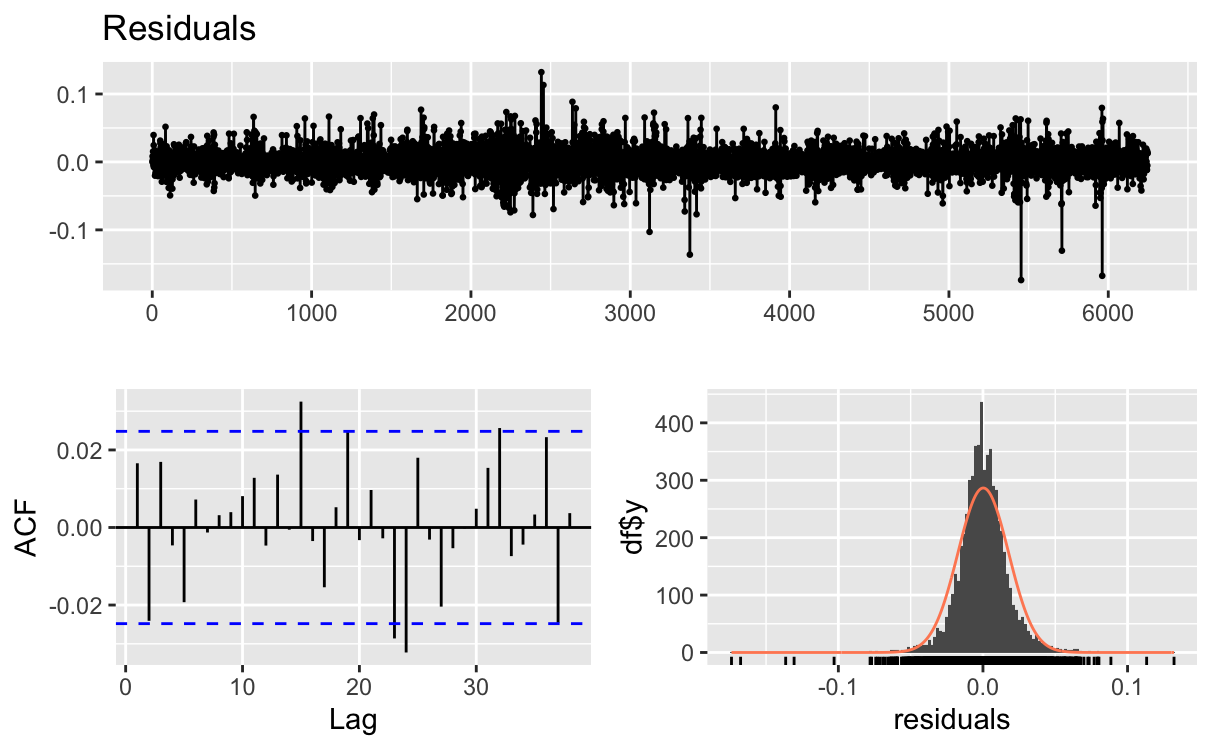
\includegraphics[width=0.85\textwidth]{figures/image25.png}\\[0.5em]
\begin{minipage}{0.48\textwidth}\centering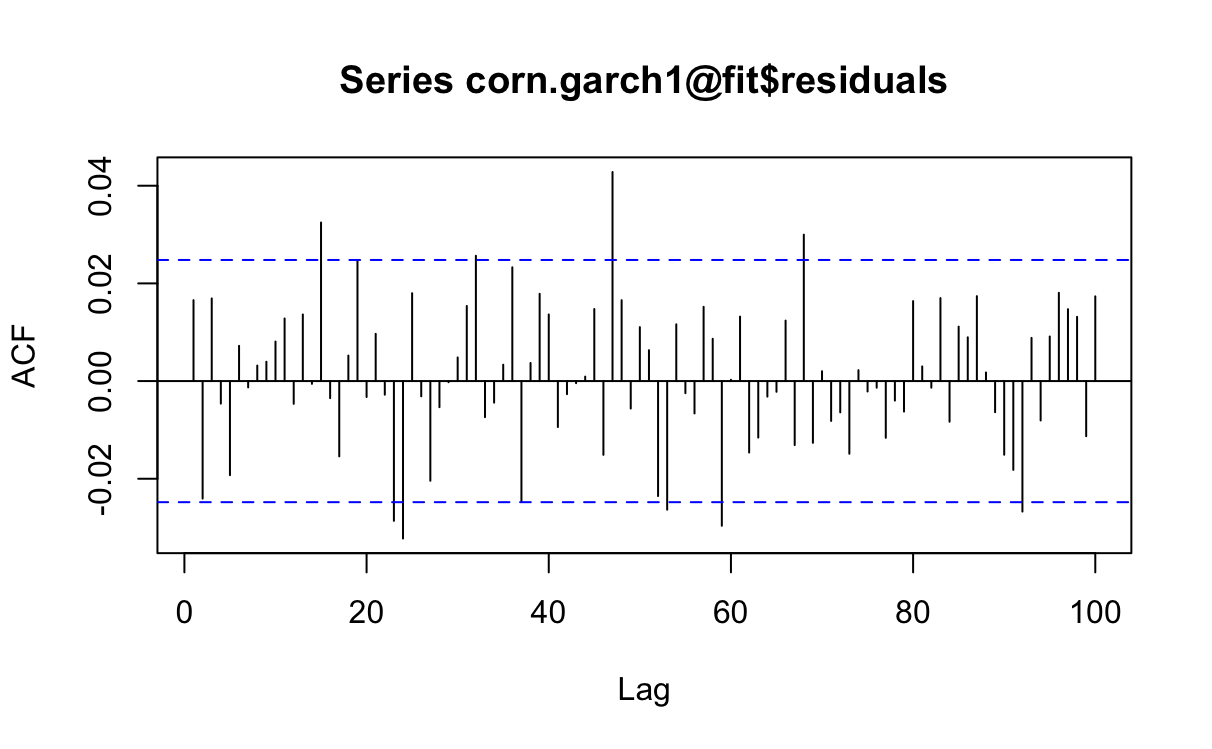
\includegraphics[width=\textwidth]{figures/image45.png}\end{minipage}
\begin{minipage}{0.48\textwidth}\centering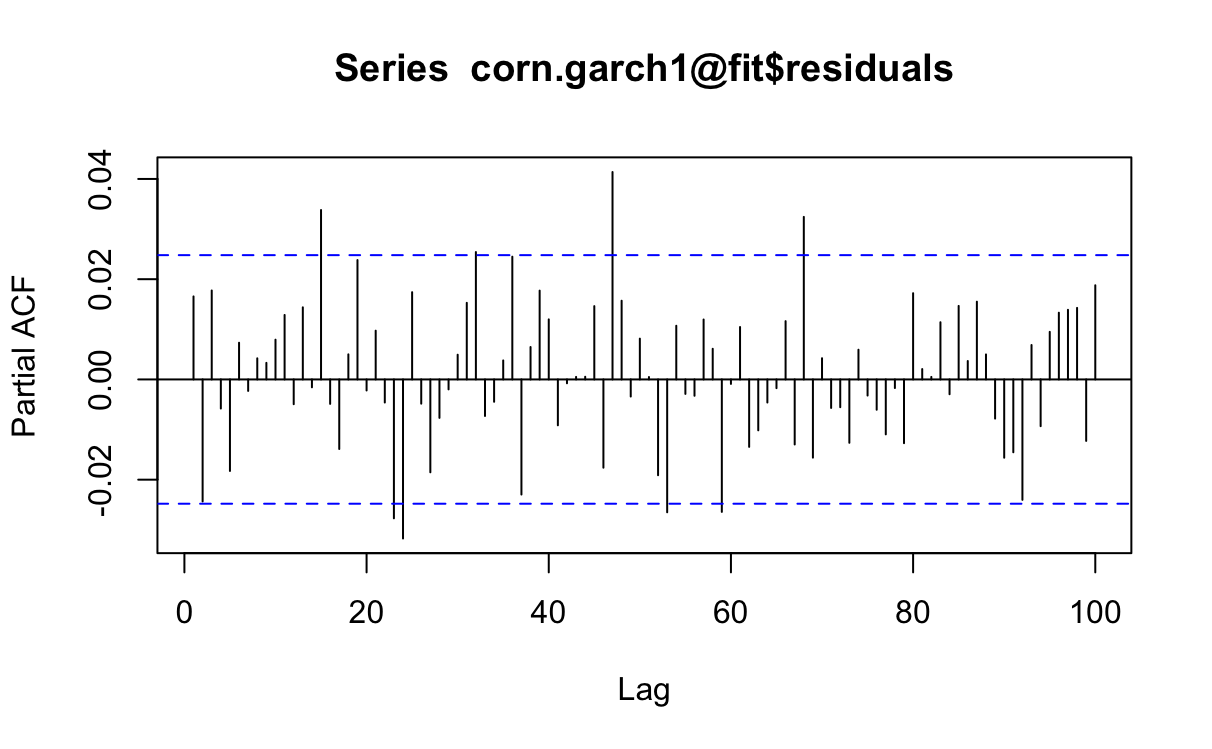
\includegraphics[width=\textwidth]{figures/image24.png}\end{minipage}

\textbf{Figure 10.} ARFIMA(0,0,0) + GARCH(1,1) with skewed Student-t distribution fitted on daily returns of US corn futures prices. The model's residuals are stationary, independent, and reasonably normal.
\end{center}
\bigskip

\begin{center}
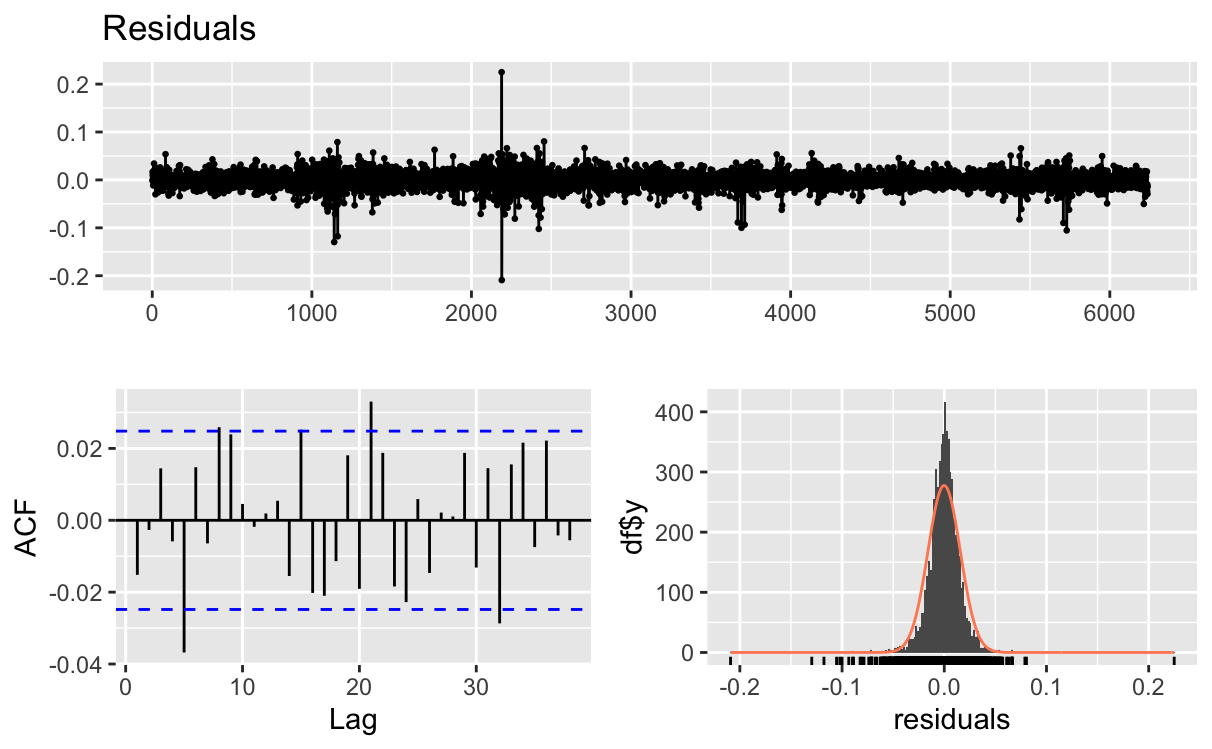
\includegraphics[width=0.85\textwidth]{figures/image15.png}\\[0.5em]
\begin{minipage}{0.48\textwidth}\centering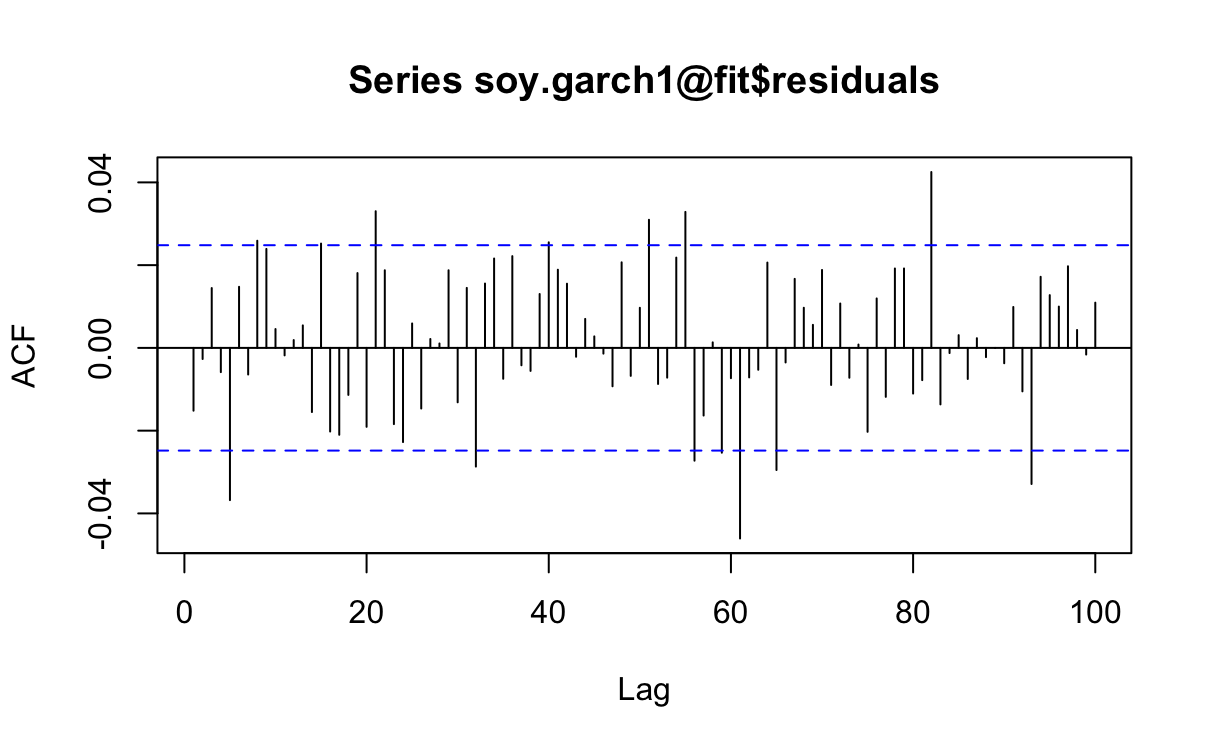
\includegraphics[width=\textwidth]{figures/image35.png}\end{minipage}
\begin{minipage}{0.48\textwidth}\centering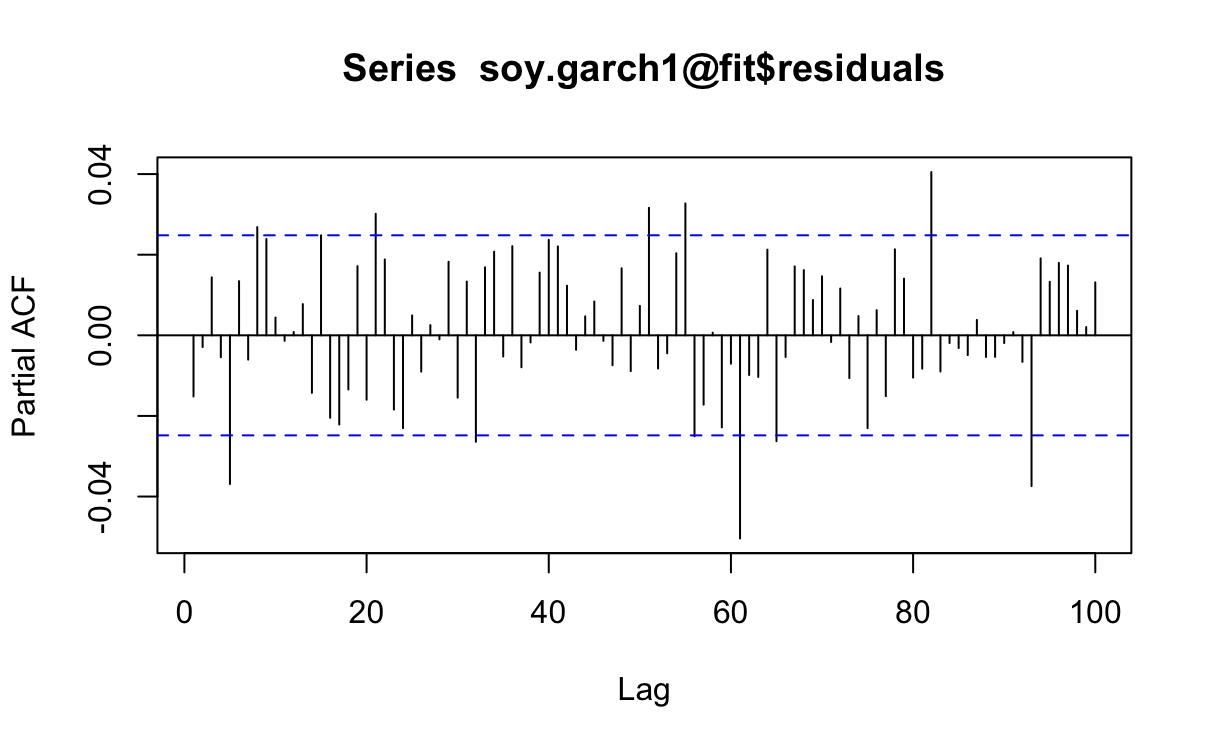
\includegraphics[width=\textwidth]{figures/image4.png}\end{minipage}

\textbf{Figure 11.} ARFIMA(0,0,0) + GARCH(1,1) with skewed Student-t distribution fitted on daily returns of US soybean futures prices. The model's residuals are stationary, acceptably independent, and reasonably normal.
\end{center}
\bigskip

\begin{center}
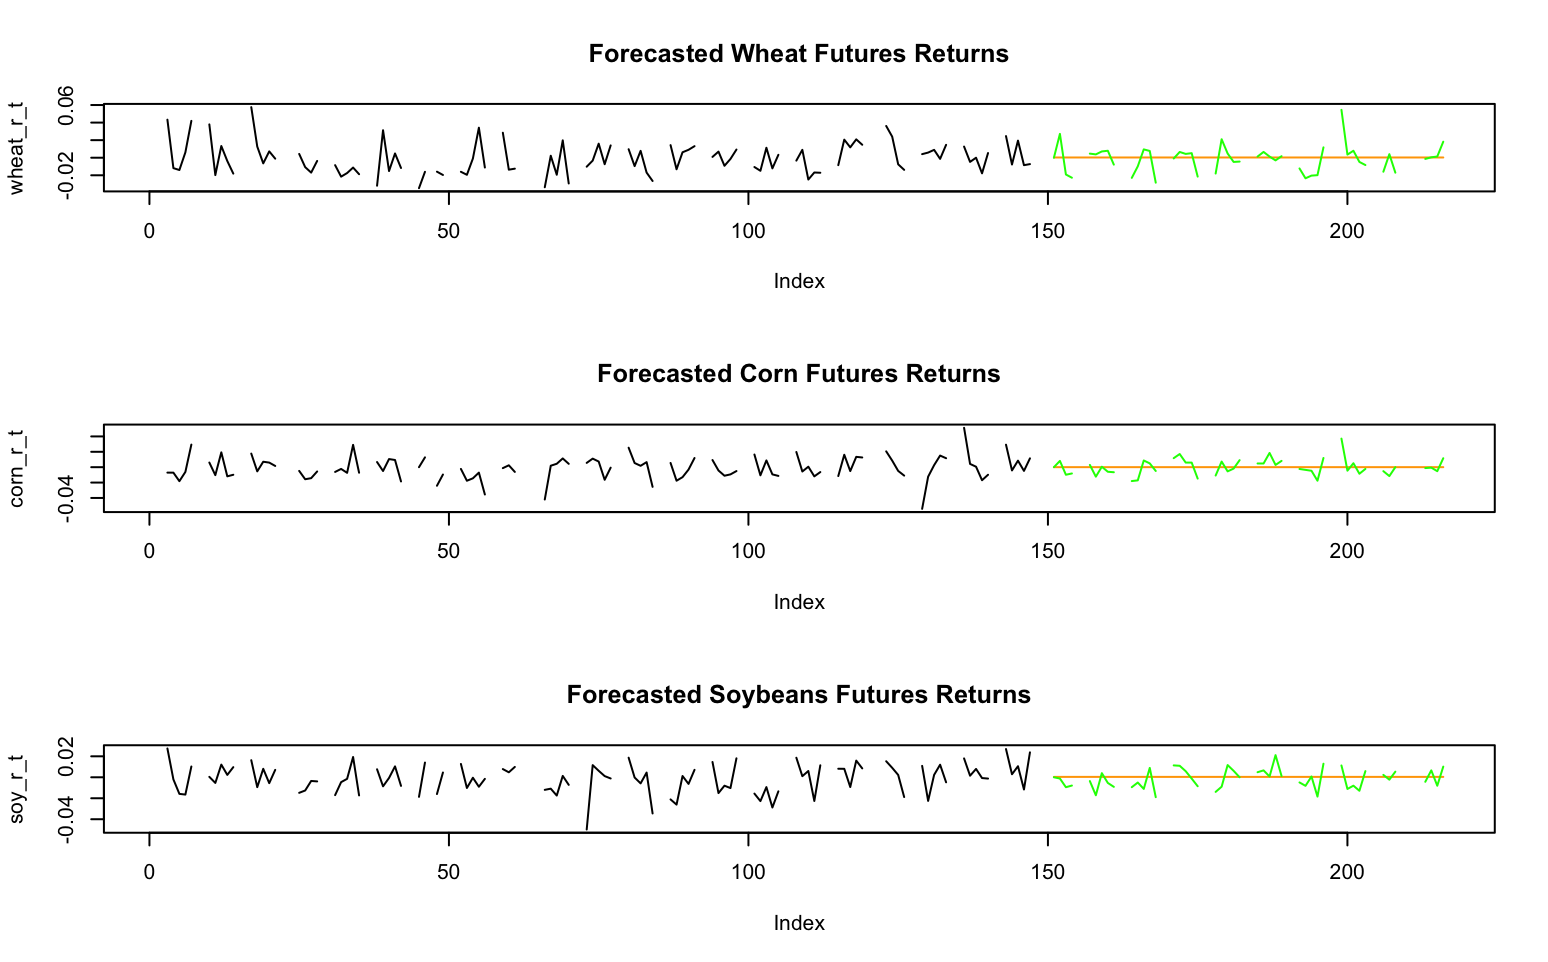
\includegraphics[width=0.9\textwidth]{figures/image6.png}

\textbf{Figure 12.} Cross Validation for GARCH models on Returns of Wheat, Corn, and Soybean Futures. R-Squared Values, respectively, are \hl{-0.0123, -9e-04}, and \hl{-0.0329}.
\end{center}
\bigskip

\begin{center}
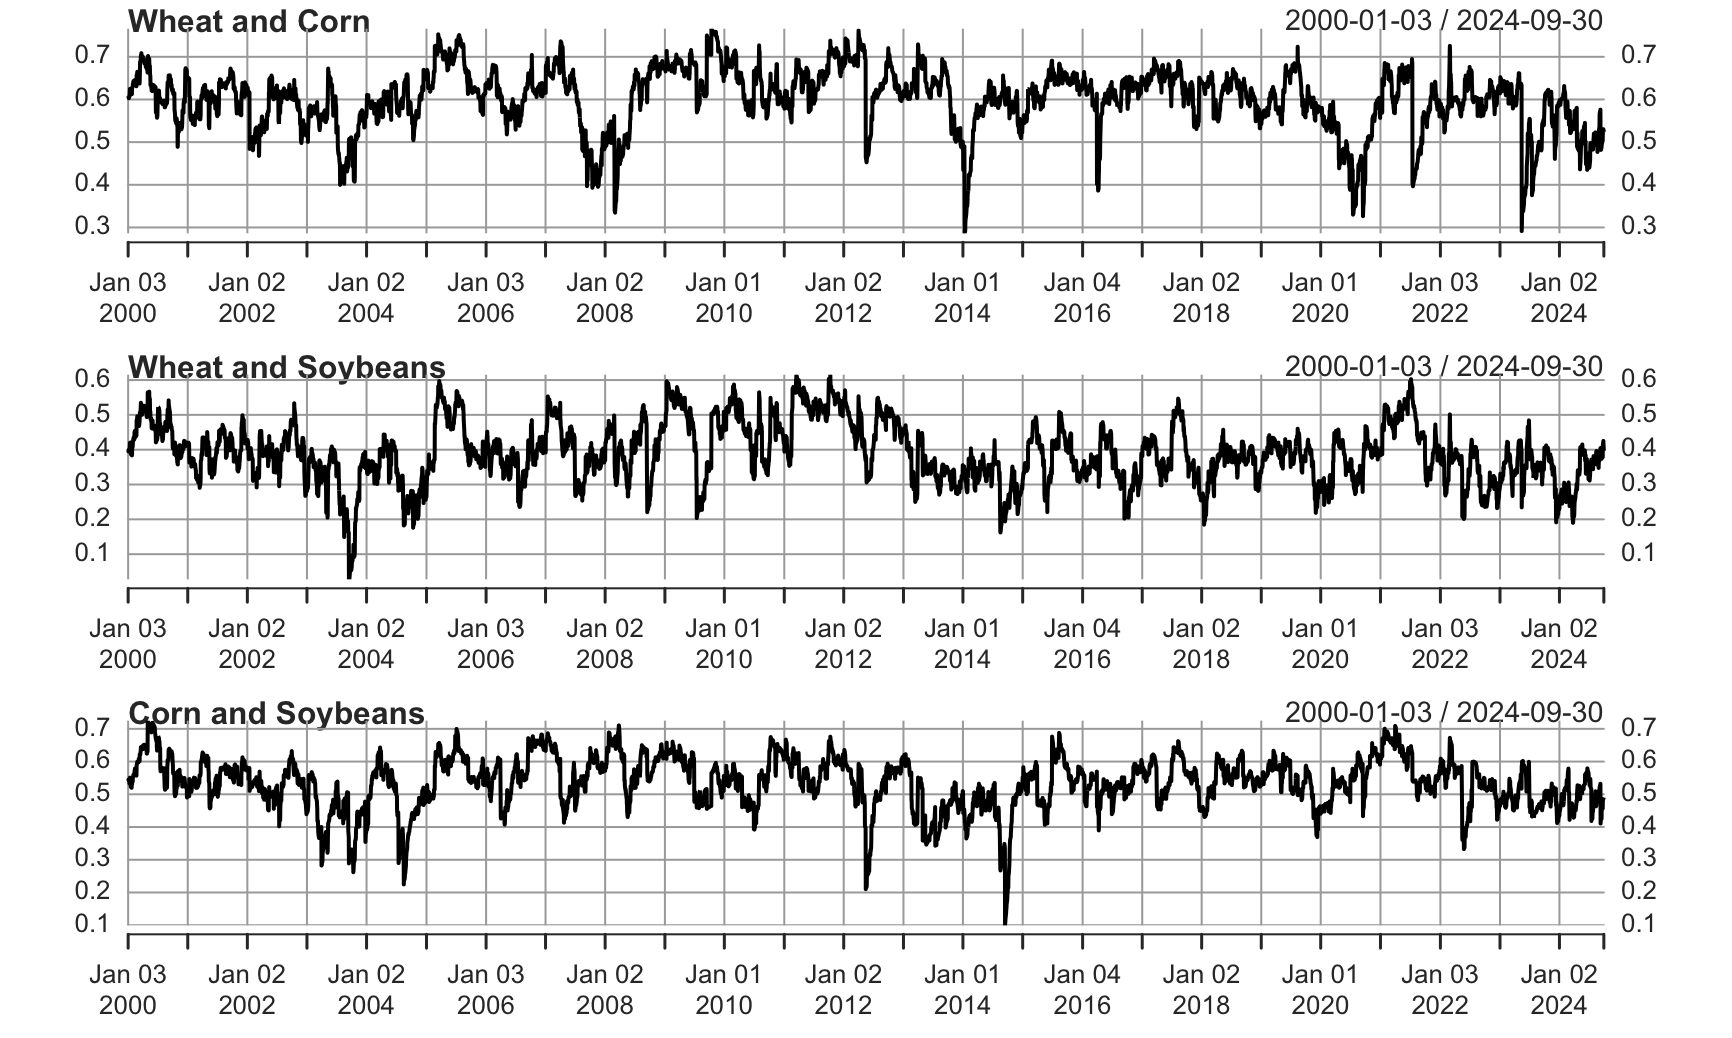
\includegraphics[width=\textwidth]{figures/image26.png}

\textbf{Figure 13.} Correlation between each pair of commodity futures over time.
\end{center}
\bigskip

\begin{center}
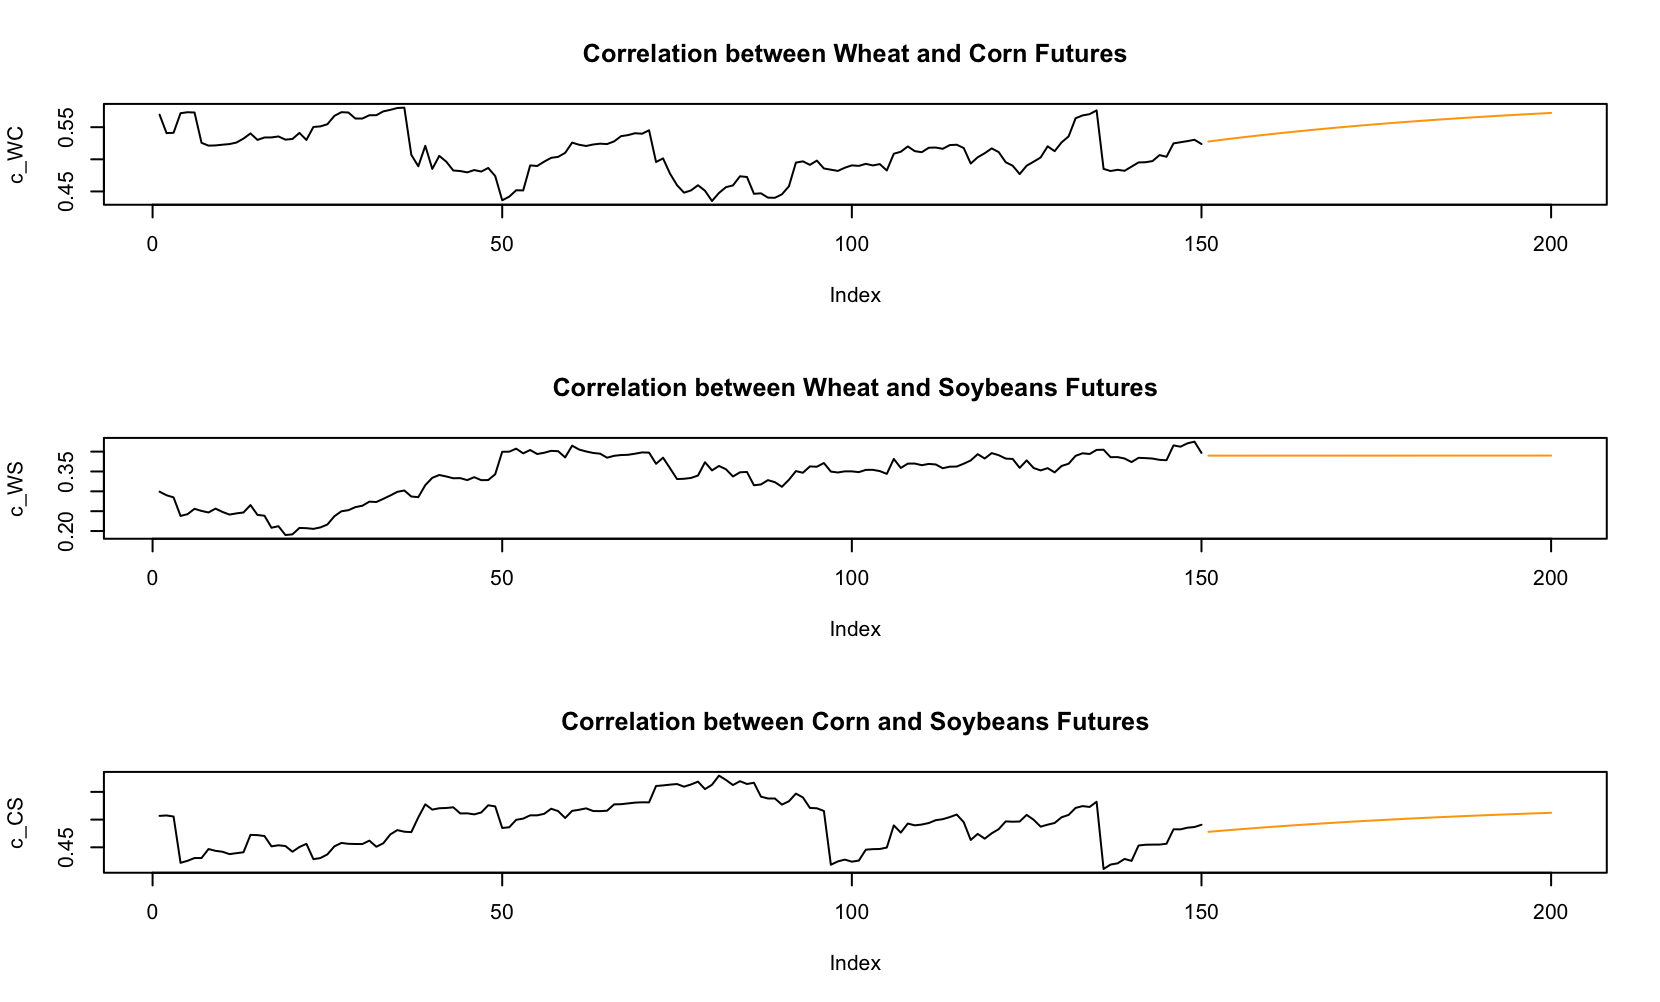
\includegraphics[width=\textwidth]{figures/image3.png}

\textbf{Figure 14.} Forecasted correlation between each pair of commodity futures over time.
\end{center}
\bigskip

\begin{center}
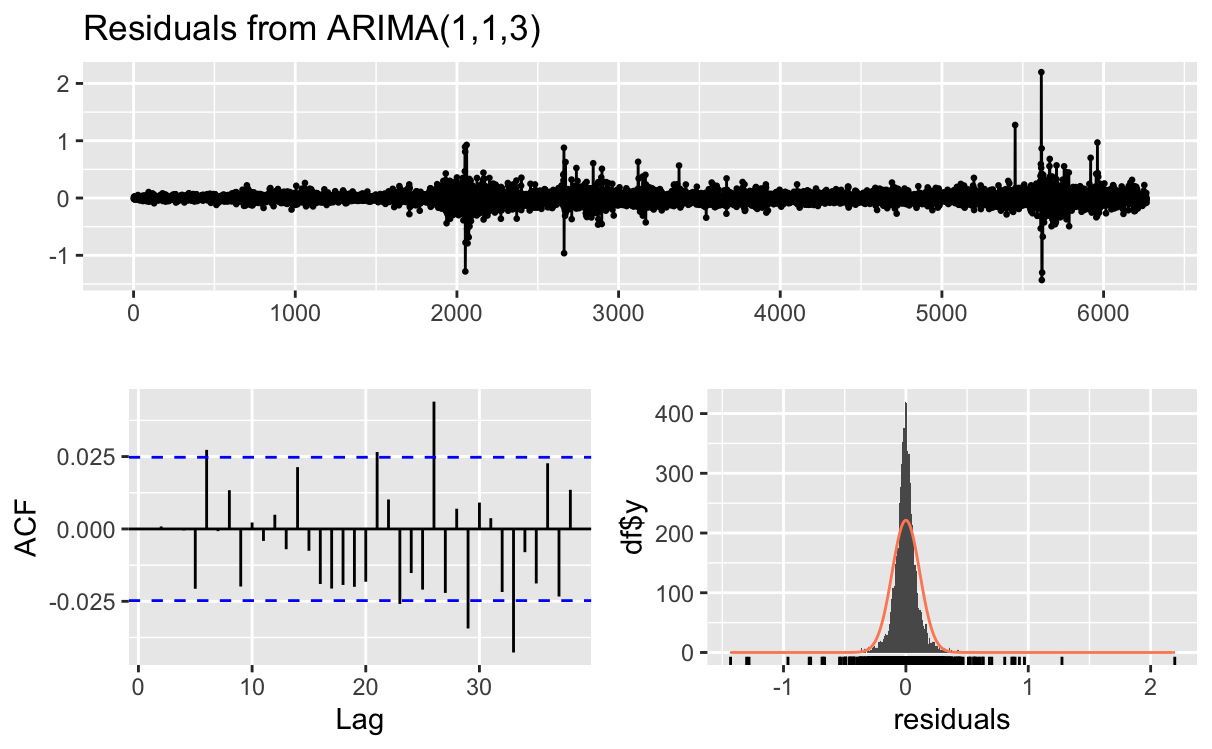
\includegraphics[width=0.85\textwidth]{figures/image36.png}

\textbf{Figure 15.} ARIMA(1,1,3)+Xreg=corn.ts model fitted on daily wheat futures prices. The residuals are stationary and independent (Ljung-Box test), but not normal, making it inappropriate for forecasting.
\end{center}
\bigskip

\begin{center}
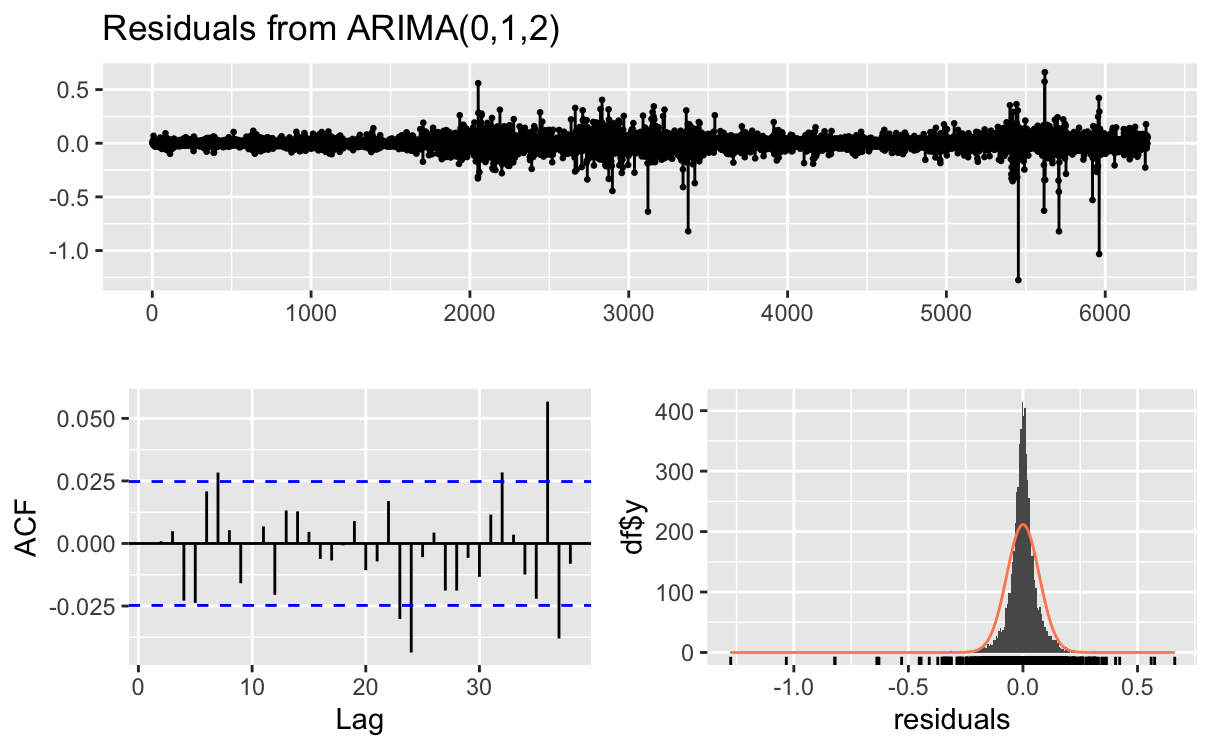
\includegraphics[width=0.9\textwidth]{figures/image12.png}

\textbf{Figure 16.} ARIMA(0,1,2)+Xreg=wheat.ts model fitted on daily corn futures prices. The residuals are stationary, but not independent (Ljung-Box test) and not normal, making it inappropriate for forecasting.
\end{center}
\skip

\begin{center}
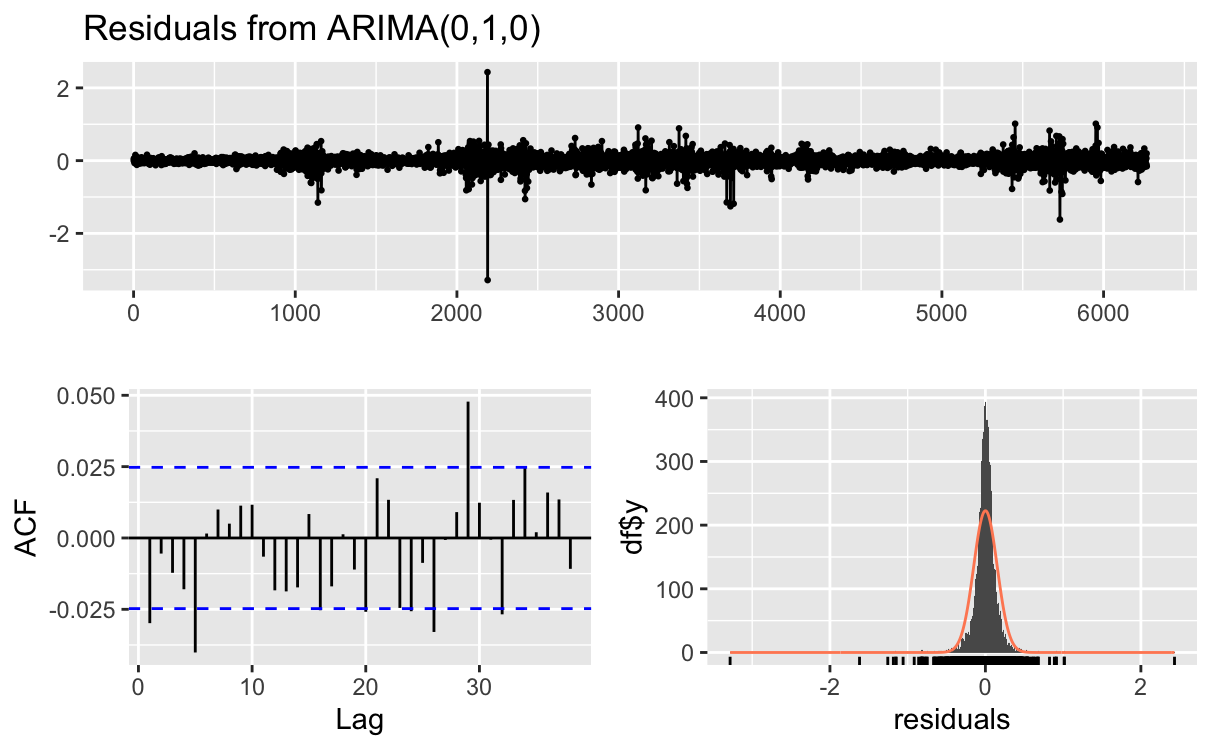
\includegraphics[width=0.9\textwidth]{figures/image31.png}

\textbf{Figure 17.} ARIMA(0,1,0)+Xreg=corn.ts model fitted on daily soybeans futures prices. The residuals are stationary, but not independent (Ljung-Box test) and not normal, making it inappropriate for forecasting.
\end{center}

\clearpage

% ==================================================================
\section{References}
% ==================================================================

\begin{references}

\item ``Chicago SRW Wheat Futures, Dec-2 (ZW=F) Stock Historical Prices \& Data - Yahoo Finance.'' 2024. Yahoo.com. 2024. \url{https://finance.yahoo.com/quote/ZW\%3DF/history/}.

\item ``Definition of a Futures Contract - CME Group.'' 2024. @CMEGroup. 2024. \url{https://www.cmegroup.com/education/courses/introduction-to-futures/definition-of-a-futures-contract.html}.

\item Ghalanos, Alexios. 2022. ``The Rmgarch Models: Background and Properties. (Version 1.3-0).'' \url{https://cran.r-project.org/web/packages/rmgarch/vignettes/The_rmgarch_models.pdf}.

\item Hayes, Adam. 2024. ``Futures Contract.'' Investopedia. February 9, 2024. \url{https://www.investopedia.com/terms/f/futurescontract.asp}.

\item Hobby, Jolyon. 2022. ``Looking beyond the Record-Breaking Wheat Market of 2021.'' Czapp. January 13, 2022. \url{https://www.czapp.com/analyst-insights/looking-beyond-the-record-breaking-wheat-market-of-2021/}.

\item M. Ates, Aaron, Christele Marsh, and Todd Hubbs. 2024. ``Corn and Other Feed Grains.'' USDA ERS. U.S. Department of Agriculture -- Economic Research Service. June 6, 2024. \url{https://www.ers.usda.gov/topics/crops/corn-and-other-feed-grains/}.

\item Pawlowski, Piotr, Roland Rechtsteiner, and Joscha Schabram. 2024. ``The Critical Role of Commodity Trading in Times of Uncertainty.'' McKinsey \& Company. April 4, 2024. \url{https://www.mckinsey.com/industries/electric-power-and-natural-gas/our-insights/the-critical-role-of-commodity-trading-in-times-of-uncertainty}.

\item Silvennoinen, Annastiina, and Timo Ter\"asvirta. 2008. ``Multivariate GARCH Models.'' SSE/EFI Working Paper Series in Economics and Finance, no. 669 (January). \url{http://hdl.handle.net/10419/56218}.

\item ``US Corn Futures Historical Prices.'' n.d. Investing.com. \url{https://www.investing.com/commodities/us-corn-historical-data}.

\item ``US Wheat Futures Historical Prices.'' 2023. Investing.com. September 20, 2023. \url{https://www.investing.com/commodities/us-wheat-historical-data}.

\item ``What Is an ARIMAX Model?'' 2024. GeeksforGeeks. June 3, 2024. \url{https://www.geeksforgeeks.org/what-is-an-arimax-model/}.

\end{references}

\end{document}
